\section{Evaluation Results and Analysis}
\label{sec:experiment_results}

We answer the four questions in Section~\ref{sec:experimental_scheme} one by one with experiments.
%
Without otherwise mentioned, the reported training time per epoch was the average wall-clock training time of 50 epochs, excluding abnormal epochs.
%
During the training of some epochs, there were extra profiling overheads from NVIDIA Nsight Systems and GC pauses from the Python interpreter that significantly increased the training time.
%
We denoted the 25\% and 75\% quantiles of the training time of 50 epochs as Q1 and Q3, respectively.
%
We regarded the epochs with the training time \emph{outside} the range of $[Q1 - 1.5 * (Q3-Q1), Q3 + 1.5 * (Q3-Q1)]$ as abnormal epochs.

\subsection{Effects of Hyper-parameters on Performance}
\label{sec:effects_of_hyper-parameters_on_performance}

The hyper-parameters of a GNN (such as the dimensions of hidden vectors and the number of heads) determined the model complexity of the GNN.
%
They affected the training/inference time, memory usage, and accuracy of the GNN at the same time.


\subsubsection{Effects on Training Time}

According to \tablename~\ref{tab:gnn_overview_edge} and \tablename~\ref{tab:gnn_overview_vertex}, the time complexity of the messaging function $\phi$ and the updating function $\gamma$ was linear to each hyper-parameter separately.
%
If we increased one of the hyper-parameters and fixed the others, the training time should increase linearly in theory.

To verify the time complexity analysis in \tablename~\ref{tab:gnn_overview_edge} and \tablename~\ref{tab:gnn_overview_vertex}, we first compared the {training} time of the four GNNs in \figurename~\ref{fig:exp_absolute_training_time}.
%
The ranking of the training time was GaAN $\gg$ GAT $>$ GGNN $>$ GCN in all cases.
%
Since the real-world graphs had more edges than vertices ($|\mathcal{E}| > |\mathcal{V}|$), the time complexity of the edge calculation stage affected more obviously than the vertex calculation stage.
%
The ranking was consistent with the time complexity analysis.

\begin{figure}[H]
    \centering
    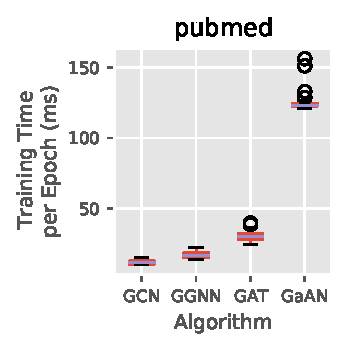
\includegraphics[width=0.3\textwidth]{figs/experiments/exp_absolute_training_time_comparison_pubmed.pdf}
    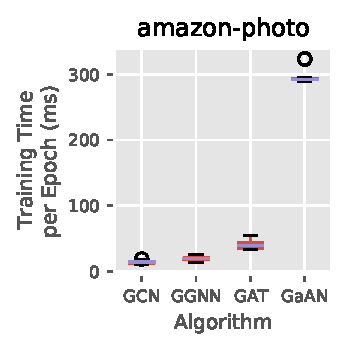
\includegraphics[width=0.3\textwidth]{figs/experiments/exp_absolute_training_time_comparison_amazon-photo.pdf}
    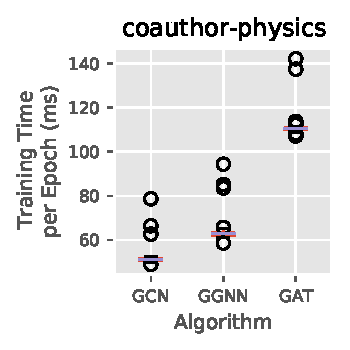
\includegraphics[width=0.3\textwidth]{figs/experiments/exp_absolute_training_time_comparison_coauthor-physics.pdf}

    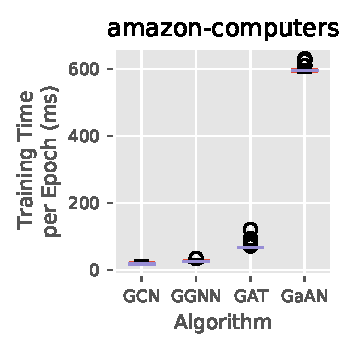
\includegraphics[width=0.3\textwidth]{figs/experiments/exp_absolute_training_time_comparison_amazon-computers.pdf}
    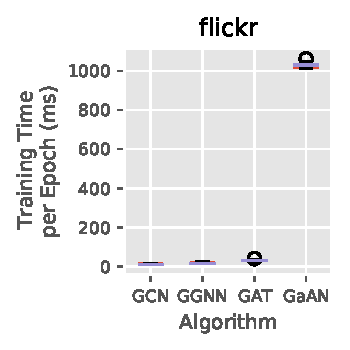
\includegraphics[width=0.3\textwidth]{figs/experiments/exp_absolute_training_time_comparison_flickr.pdf}
    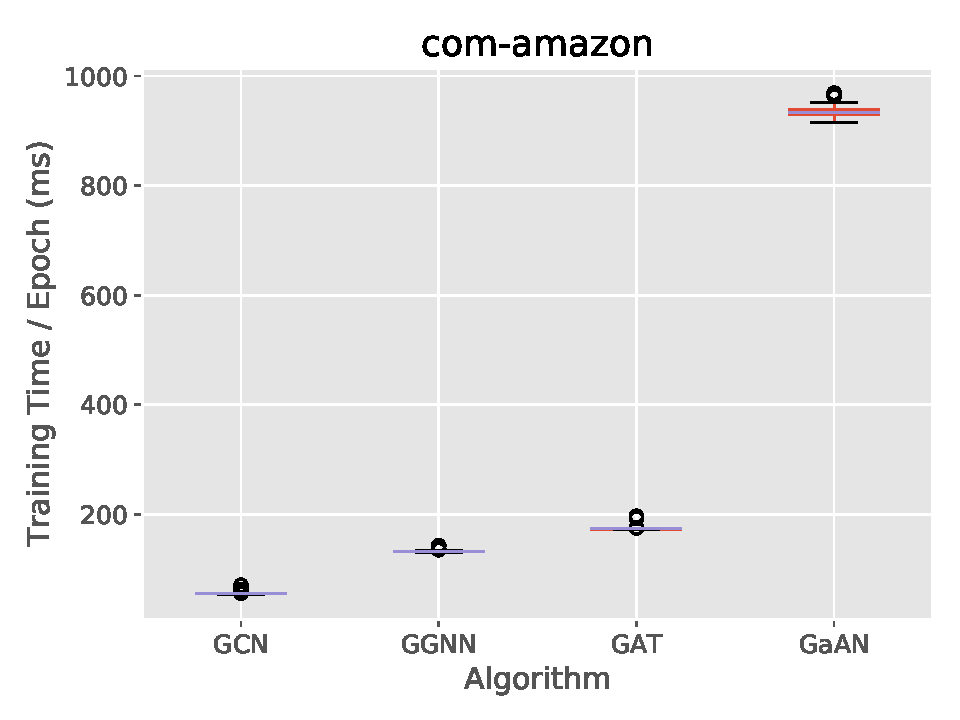
\includegraphics[width=0.3\textwidth]{figs/experiments/exp_absolute_training_time_comparison_com-amazon.pdf}
    \caption{Distribution of the wall-clock training time of 50 epochs on different datasets. GaAN crashed due to the out of memory exception on the \texttt{cph} dataset.}
    \label{fig:exp_absolute_training_time}
\end{figure}

To further evaluate effects of hyper-parameters on training time, we measured the training time of each GNN with varying hyper-parameters in \figurename~\ref{fig:exp_hyperparameter_on_vertex_edge_phase_time_gcn} to \figurename~\ref{fig:exp_hyperparameter_on_vertex_edge_phase_time_gaan}.


%\begin{figure}[H]
    %\centering
    %\subfloat[GCN\label{fig:exp_hyperparameter_on_vertex_edge_phase_time_gcn}]{\includegraphics[width=0.6\textwidth]%{figs/experiments/exp_hyperparameter_on_vertex_edge_phase_time_gcn.pdf}}
%    \\
    %\subfloat[GGNN\label{fig:exp_hyperparameter_on_vertex_edge_phase_time_ggnn}]{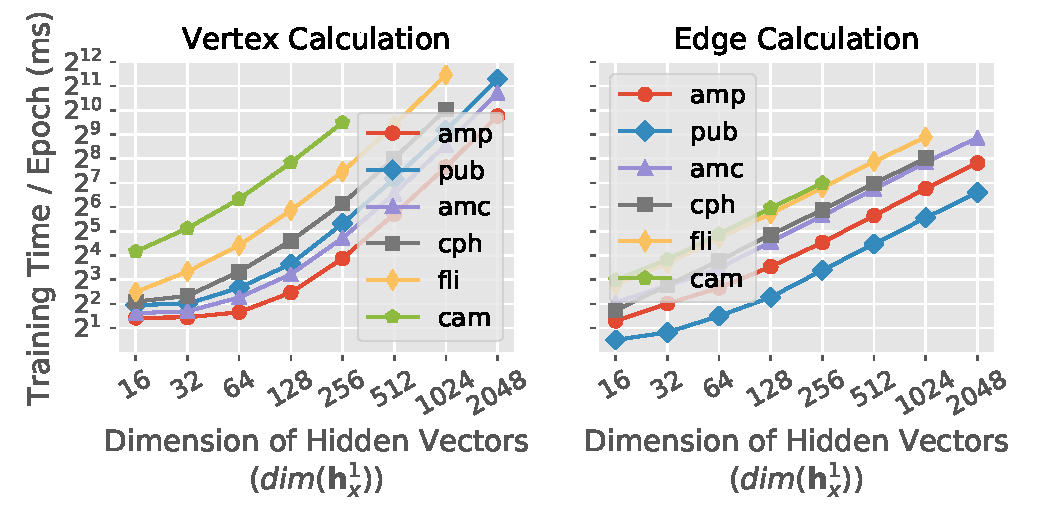
\includegraphics[width=0.6\textwidth]{figs/experiments/exp_hyperparameter_on_vertex_edge_phase_time_ggnn.pdf}}
%    \\
    %\subfloat[GAT\label{fig:exp_hyperparameter_on_vertex_edge_phase_time_gat}]{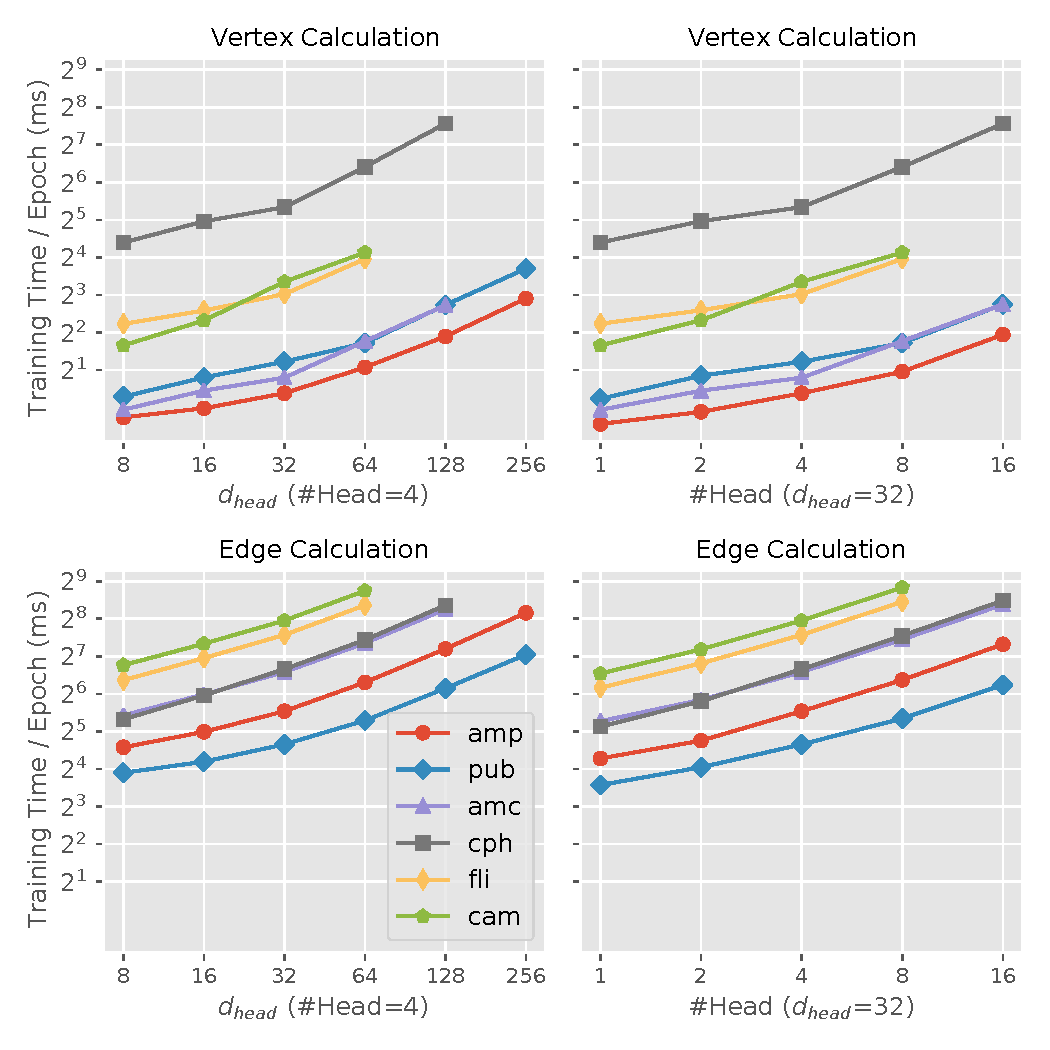
\includegraphics[width=0.6\textwidth]{figs/experiments/exp_hyperparameter_on_vertex_edge_phase_time_gat.pdf}}
    %\\
    %\subfloat[GaAN\label{fig:exp_hyperparameter_on_vertex_edge_phase_time_gaan}]{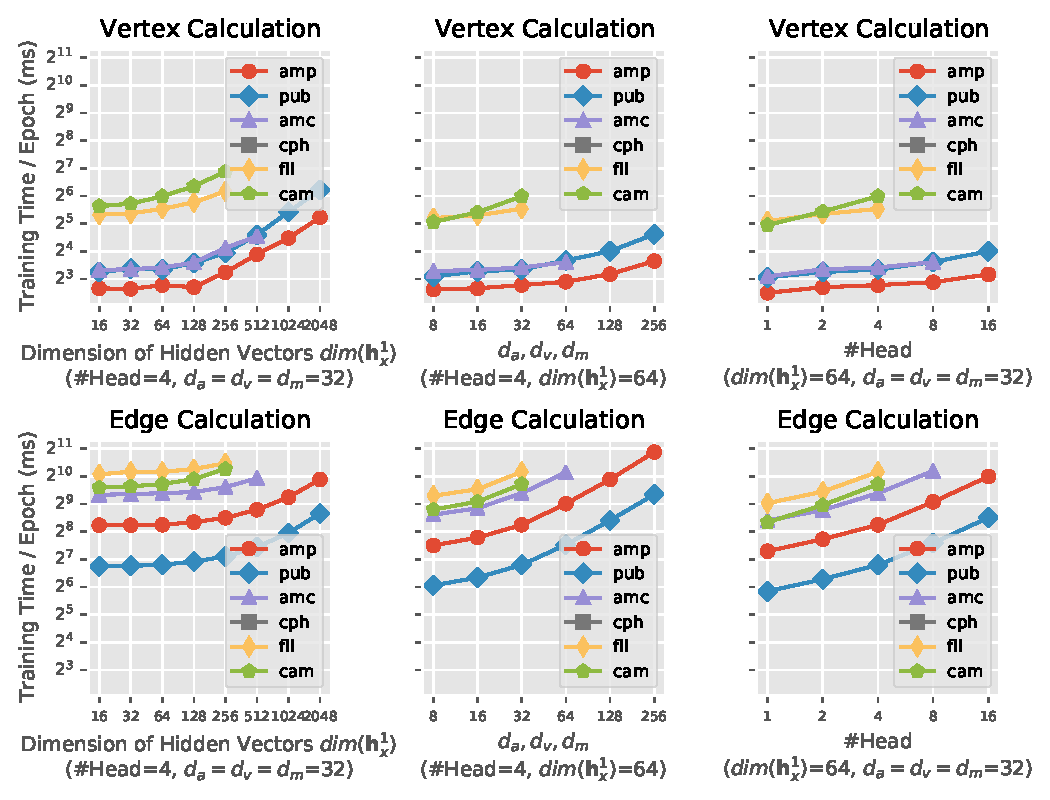
\includegraphics[width=0.9\textwidth]{figs/experiments/exp_hyperparameter_on_vertex_edge_phase_time_gaan.pdf}}

    %\caption{Effects of hyper-parameters on the edge/vertex calculation time.}
    %\label{fig:exp_hyperparameter_on_vertex_edge_phase_time}
%\end{figure}

For GCN and GGNN, $dim(\MyVec{h}^0_x)$ and $dim(\MyVec{h}^1_x)$ were solely determined by the dataset with $d^0_{in} = dim(\MyVec{h}^0_x) = dim(\MyVec{v_x})$ and $d^1_{out} = dim(\boldsymbol{h}^2_x)=\#Class$.
%
Therefore, the only modifiable hyper-parameter was the dimension of $\MyVec{h}^1_x$ that affected the dimension of output hidden vectors of the layer 0 $d^0_{out}$ and the dimension of input hidden vectors of the layer 1 $d^1_{in}$ simultaneously, i.e. $dim(\MyVec{h}^1_x)  = d^0_{out} = d^1_{in}$.
%
According to the time complexity analysis, if we fixed other hyper-parameters but only increased $dim(\boldsymbol{h}^1_x)$, the computational costs of the GNN layer 0 and the GNN layer 1 should both increase linearly with $dim(\boldsymbol{h}^1_x)$, causing the training time of the whole GNN also increased linearly. 
%
\figurename~\ref{fig:exp_hyperparameter_on_vertex_edge_phase_time_gcn} and \figurename~\ref{fig:exp_hyperparameter_on_vertex_edge_phase_time_ggnn} show that the training time of GCN and GGNN increased linearly with $dim(\boldsymbol{h}^1_x)$ when $dim(\boldsymbol{h}^1_x)$ was big, consistent with the theoretical analysis.

\begin{figure}[H]
    \centering
    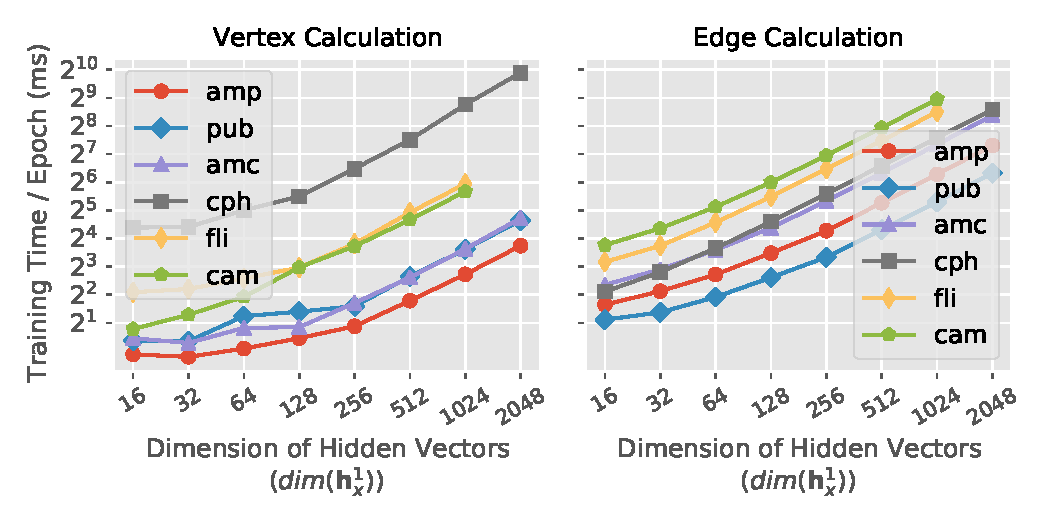
\includegraphics[width=0.6\textwidth]{figs/experiments/exp_hyperparameter_on_vertex_edge_phase_time_gcn.pdf}
    \caption{Effects of hyper-parameters on the vertex/edge calculation time of GCN in training.}
    \label{fig:exp_hyperparameter_on_vertex_edge_phase_time_gcn}
\end{figure}

\begin{figure}[H]
    \centering
    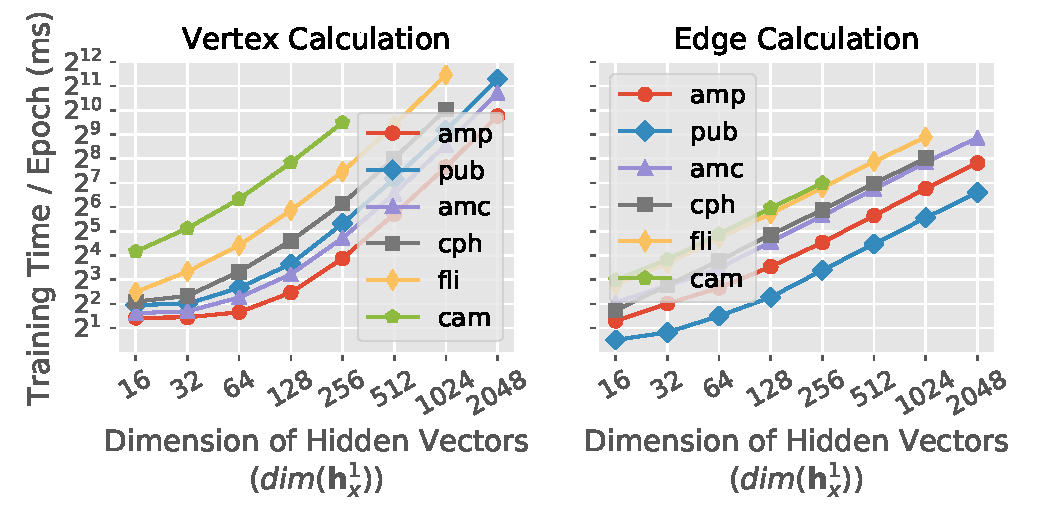
\includegraphics[width=0.6\textwidth]{figs/experiments/exp_hyperparameter_on_vertex_edge_phase_time_ggnn.pdf}
    \caption{Effects of hyper-parameters on the vertex/edge calculation time of GGNN in training.}
    \label{fig:exp_hyperparameter_on_vertex_edge_phase_time_ggnn}
\end{figure}

For GAT, we modified the number of heads $K$ and the dimension of each head $d_{head}$ in the GAT layer 0.
%
The dimension of $\MyVec{h}^1_x$ was determined as $dim(\boldsymbol{h}^1_x) = K d_{head}$.
%
Thus, the computational costs of the GAT layer 0 and the GAT layer 1 should increase linearly with $K$ and $d_{head}$ separately. 
%
\figurename~\ref{fig:exp_hyperparameter_on_vertex_edge_phase_time_gat} confirms the theoretical analysis.


\begin{figure}[H]
    \centering
    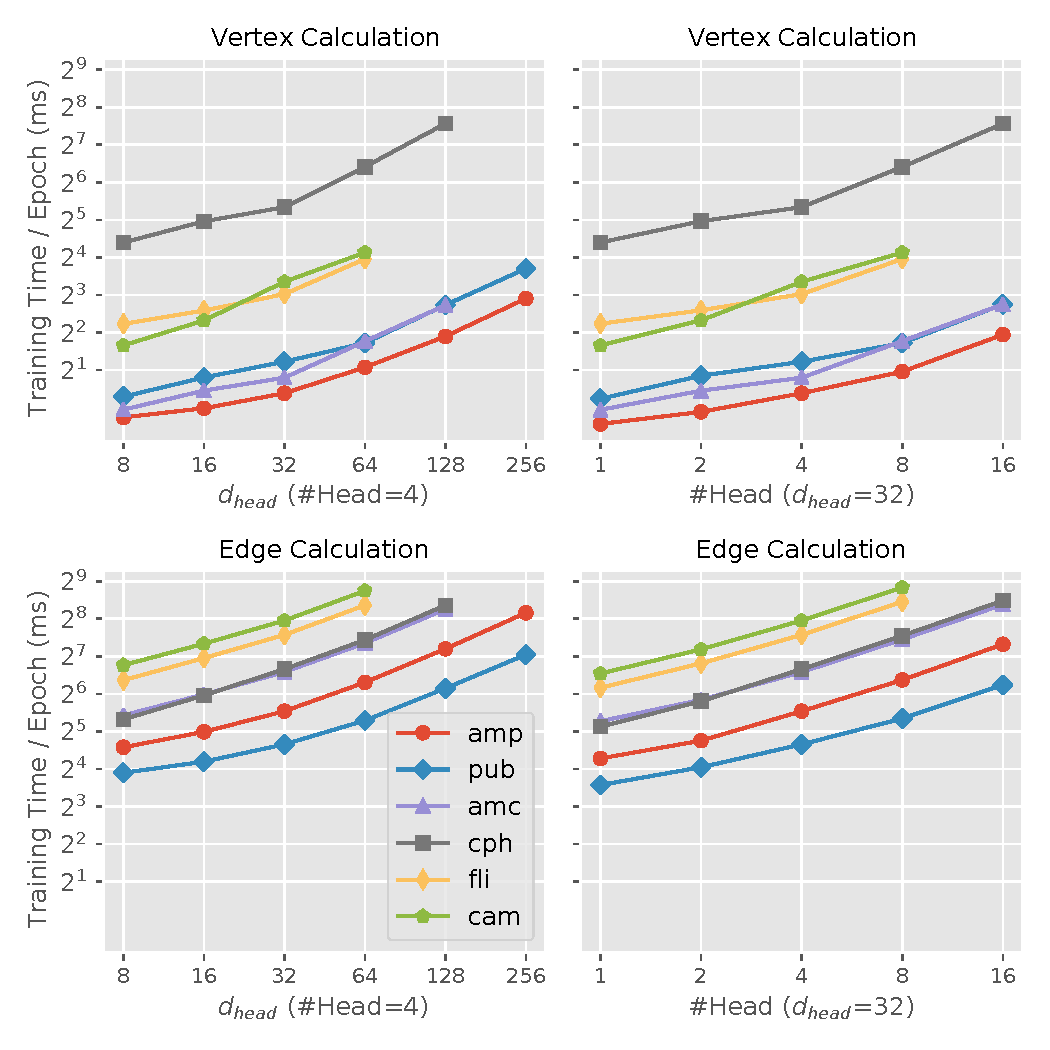
\includegraphics[width=0.6\textwidth]{figs/experiments/exp_hyperparameter_on_vertex_edge_phase_time_gat.pdf}
    \caption{Effects of hyper-parameters on the vertex/edge calculation time of GAT in training.}
    \label{fig:exp_hyperparameter_on_vertex_edge_phase_time_gat}
\end{figure}

For GaAN, it was also based on the multi-head mechanism.
%
Its time complexity should be affected by $dim(\boldsymbol{h}^1_x)$ ($d^0_{out} = d^1_{in} = dim(\boldsymbol{h}^1_x)$), $d_a$, $d_v$, $d_m$, and the number of heads $K$.
%
\figurename~\ref{fig:exp_hyperparameter_on_vertex_edge_phase_time_gaan} demonstrates that the training time increased linearly with the hyper-parameters, except for $dim(\boldsymbol{h}^1_x)$.
As $dim(\boldsymbol{h}^1_x)$ increased, the training time increased first slightly and then linearly.
We observed similar phenomena in GCN, GGNN, and GAT:
When the values of hyper-parameters were too low, GNN training could not make full use of the computing power of the GPU.
%
When the values of hyper-parameters became high enough, training time increased linearly, supporting the time complexity analysis.


\begin{figure}[H]
    \centering
    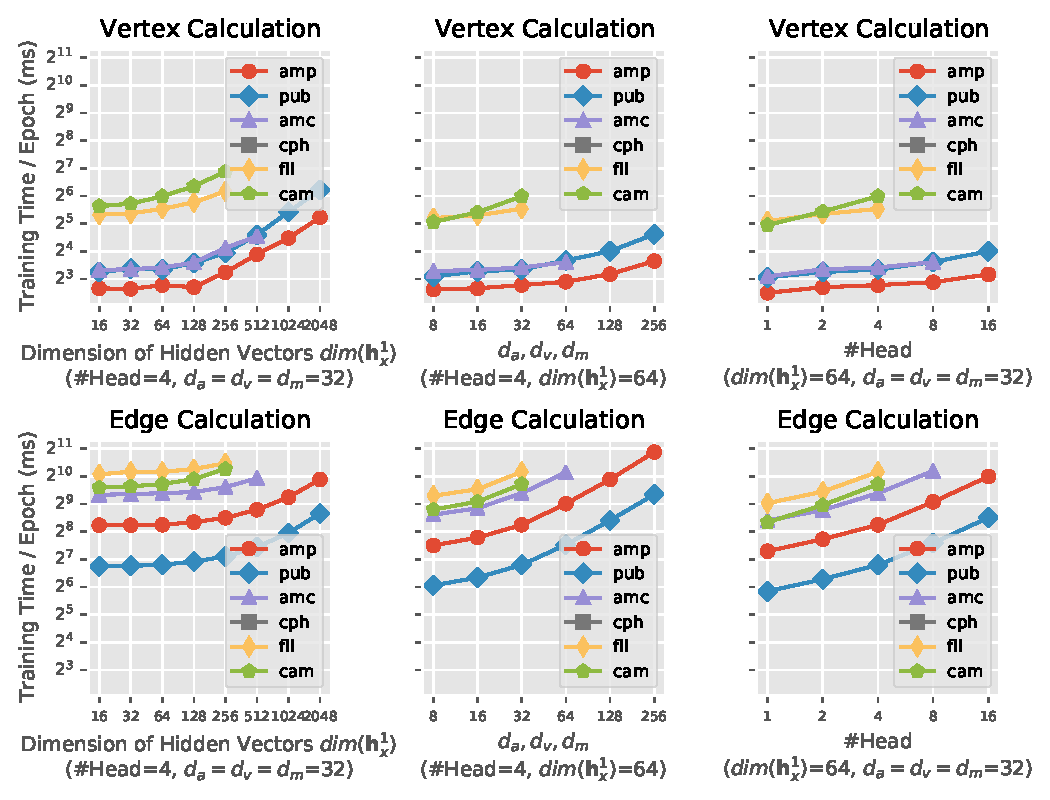
\includegraphics[width=0.8\textwidth]{figs/experiments/exp_hyperparameter_on_vertex_edge_phase_time_gaan.pdf}
    \caption{Effects of hyper-parameters on the vertex/edge calculation time of GaAN in training.}
    \label{fig:exp_hyperparameter_on_vertex_edge_phase_time_gaan}
\end{figure}

\subsubsection{Effects on Inference Time}

For all GNNs, we found that the effects of hyper-parameters on the inference time were the same as the training time.
%
Taking GGNN as an exmple, \figurename~\ref{fig:exp_hyperparameter_on_inference_vertex_edge_phase_time_ggnn} shows the effects of hyper-parameters on inference time of GGNN.
%
By cross-comparing \figurename~\ref{fig:exp_hyperparameter_on_inference_vertex_edge_phase_time_ggnn} and \figurename~\ref{fig:exp_hyperparameter_on_vertex_edge_phase_time_ggnn}, the trends of inference time and training time were the same: as $dim(\MyVec{h}^1_x)$ increased, the vertex and edge calculation time both grew linearly when $dim(\MyVec{h}^1_x)$ was large enough.
%
For the other GNNs, we observed similar phenomena.
%
The results indicated that the complexity analysis presented in \tablename~\ref{tab:gnn_overview_edge} and \tablename~\ref{tab:gnn_overview_vertex} were also applicable to inference.

\begin{figure}[H]
    \centering
    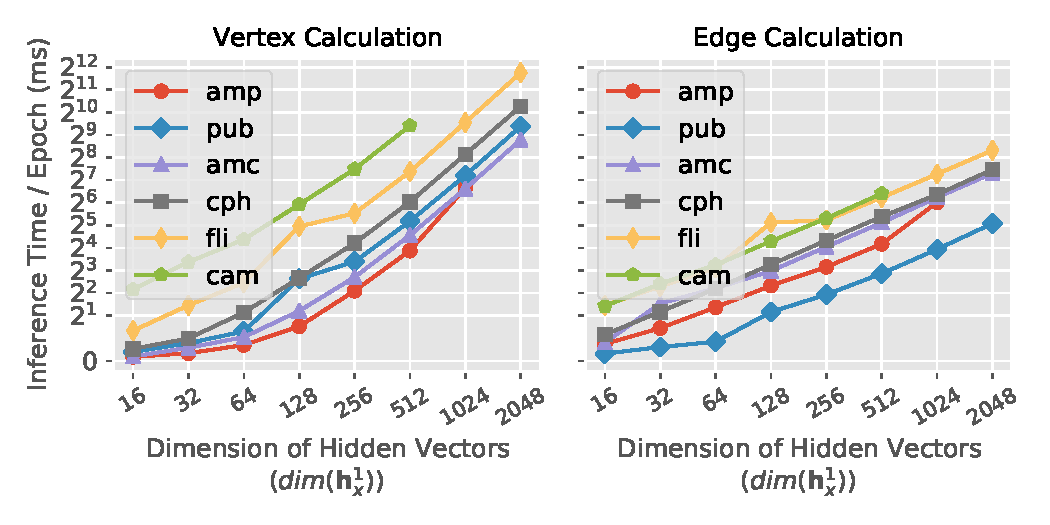
\includegraphics[width=0.6\textwidth]{figs/experiments/exp_hyperparameter_on_inference_vertex_edge_phase_time_ggnn.pdf}
    \caption{Effects of hyper-parameters on the vertex/edge calculation time of GGNN in inference.}
    \label{fig:exp_hyperparameter_on_inference_vertex_edge_phase_time_ggnn}
\end{figure}


\subsubsection{Effects on Peak Memory Usage}

We further measured the effects of the hyper-parameters on the peak GPU memory usage during training in \figurename~\ref{fig:exp_hyperparameter_memory_usage}.
%
The memory usage also increased linearly as the hyper-parameters increased for all GNNs, except for GaAN on $dim(\MyVec{h}^1_x)$.
%
As the hidden vectors $\MyVec{h}^1_x$ in GaAN consumed a small proportion of memory, the growth in the memory usage was not noticeable until $dim(\boldsymbol{h}^1_x)$ was large enough.
%
The effects of the hyper-parameters on inference memory usage were the same as training.
%
Taking GAT as an example, \figurename~\ref{fig:exp_inference_hyperparameter_memory_usage_gat} shows that the peak memory usage during inference grew linearly with the increasing hyper-parameters.
%
By cross-comparing \figurename~\ref{fig:exp_inference_hyperparameter_memory_usage_gat} and \figurename~\ref{fig:exp_hyperparameter_memory_usage_gat}, the hyper-parameters affected the peak memory usage of training and inference in the same way.
%
For the other GNNs, we observed similar phenomena.

\begin{figure}[H]
    \centering
    \subfloat[GCN]{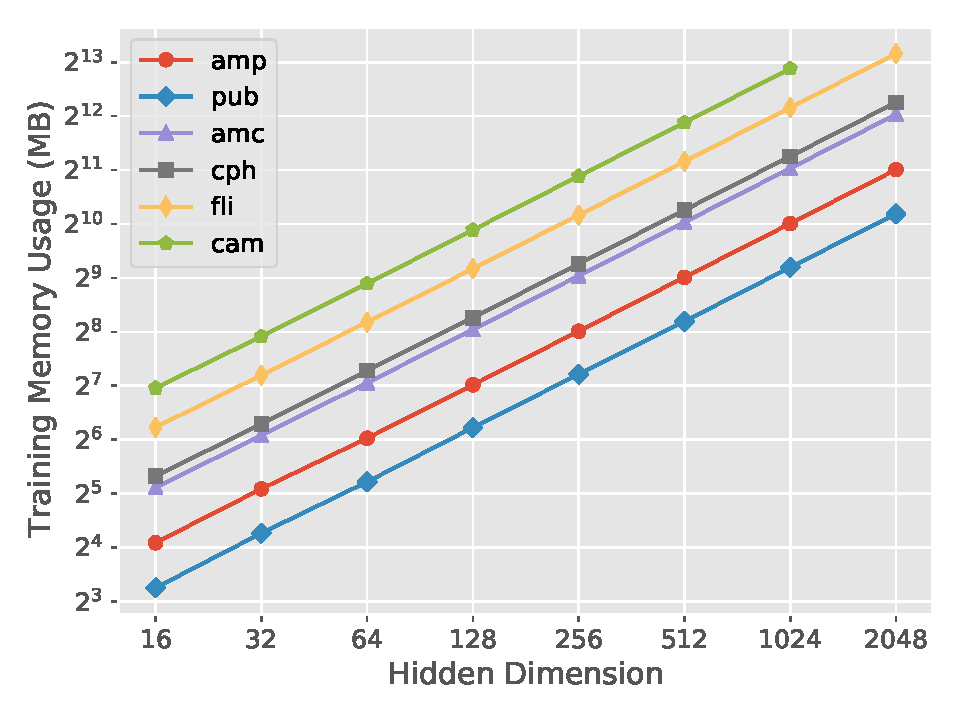
\includegraphics[width=0.25\columnwidth]{figs/experiments/exp_hyperparameter_on_memory_usage_gcn.pdf}}
    \subfloat[GGNN]{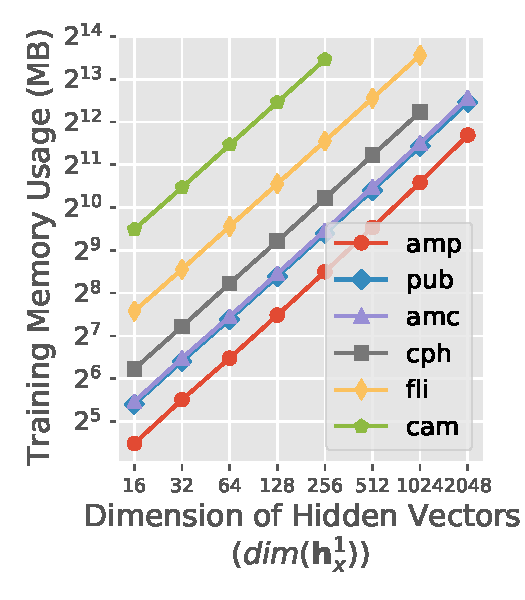
\includegraphics[width=0.25\columnwidth]{figs/experiments/exp_hyperparameter_on_memory_usage_ggnn.pdf}}
    \subfloat[GAT\label{fig:exp_hyperparameter_memory_usage_gat}]{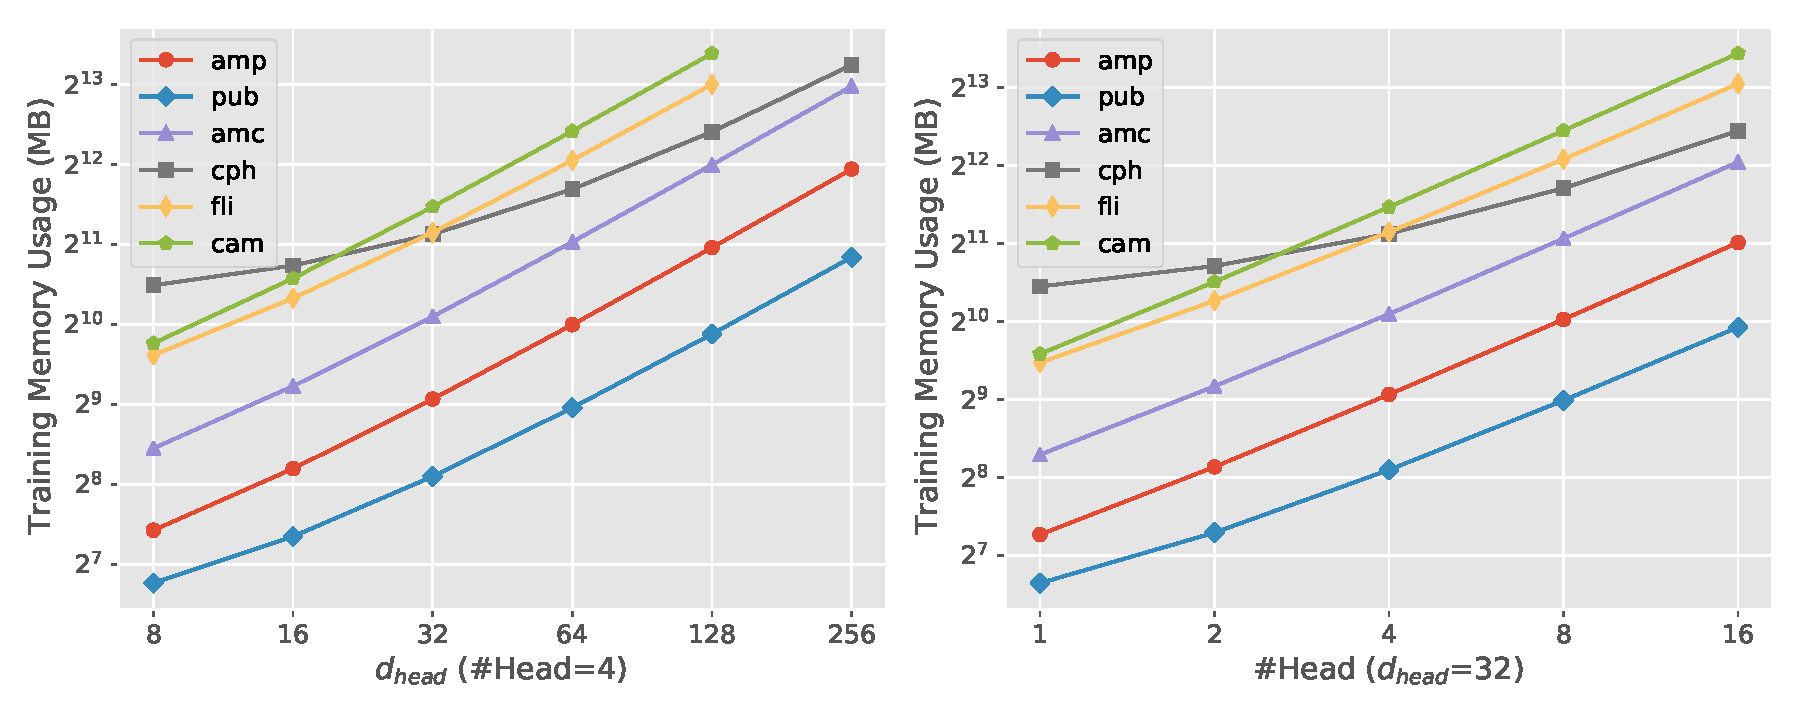
\includegraphics[width=0.5\columnwidth]{figs/experiments/exp_hyperparameter_on_memory_usage_gat.pdf}}\\
    \subfloat[GaAN]{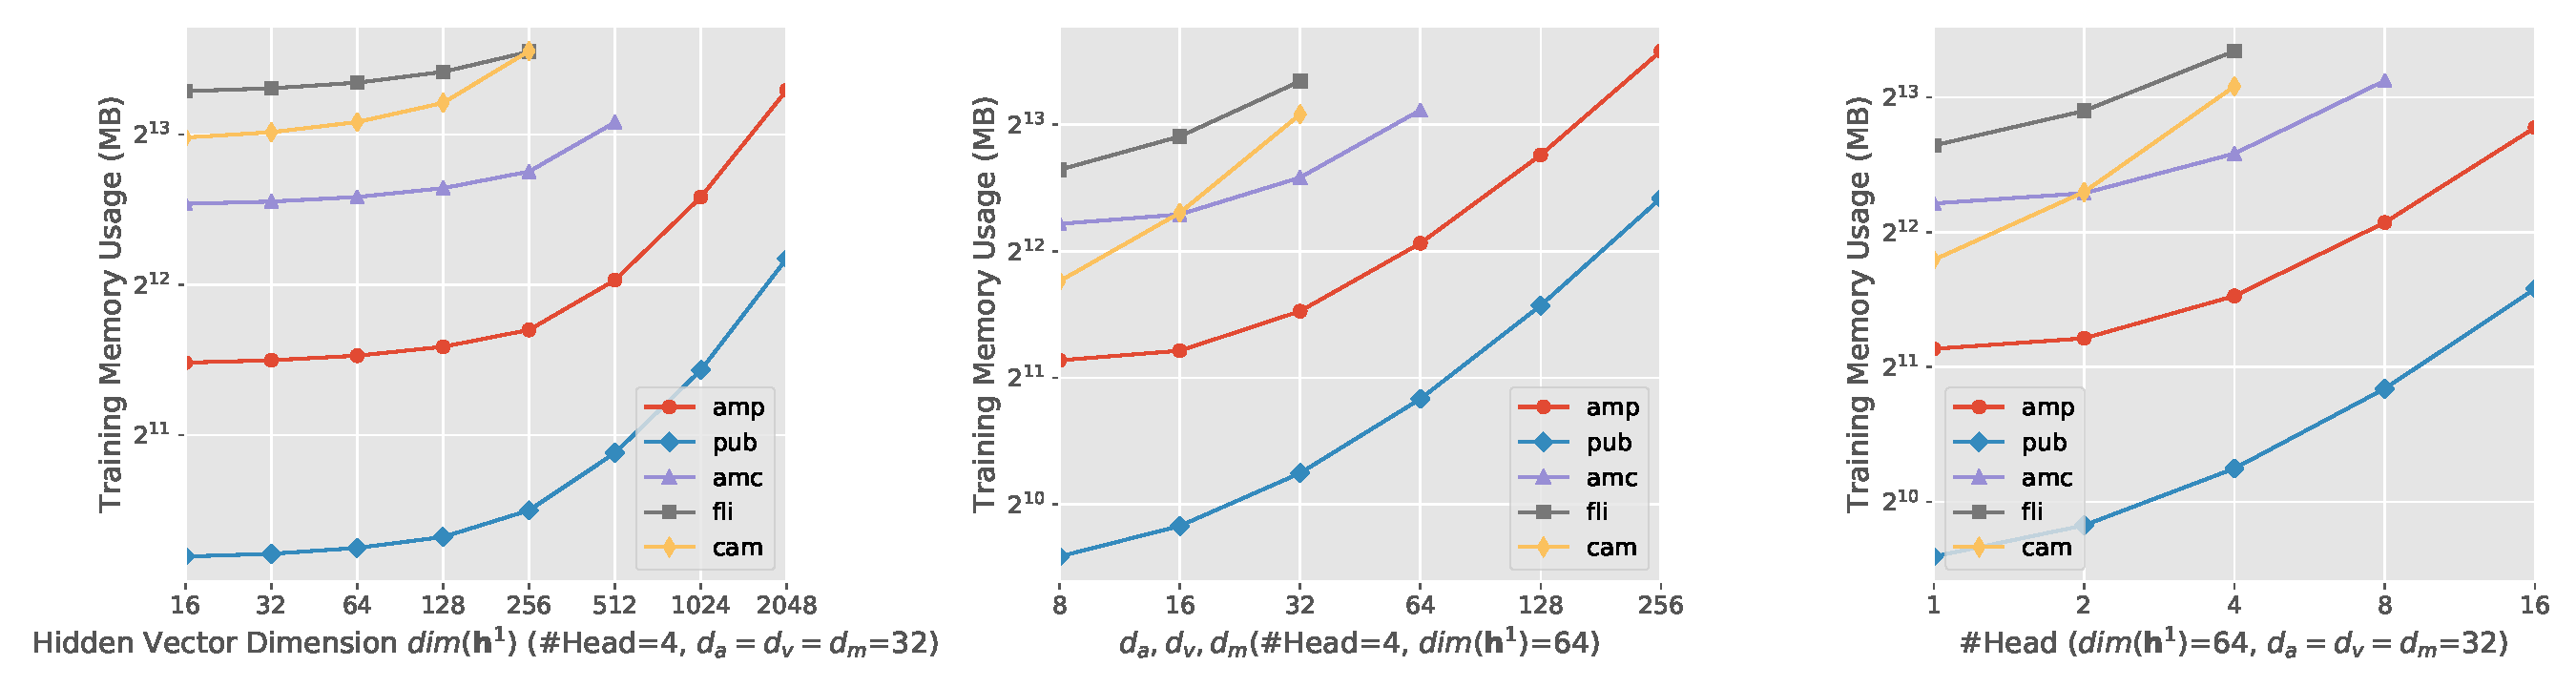
\includegraphics[width=0.75\columnwidth]{figs/experiments/exp_hyperparameter_on_memory_usage_gaan.pdf}}
    \caption{Effects of hyper-parameters on the peak GPU memory usage during training, excluding the memory used by the dataset and the model parameters.}
    \label{fig:exp_hyperparameter_memory_usage}
\end{figure}

\begin{figure}[h]
    \centering
    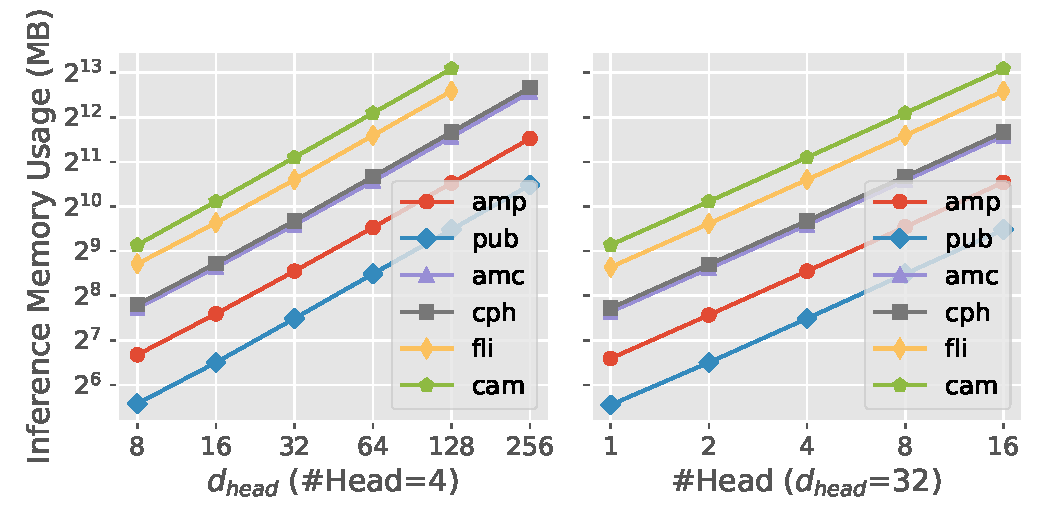
\includegraphics[width=0.5\columnwidth]{figs/experiments/exp_hyperparameter_on_inference_memory_usage_gat.pdf}
    \caption{Effects of hyper-parameters on the peak GPU memory usage during inference of GAT, excluding the memory used by the dataset and the model parameters.}
    \label{fig:exp_inference_hyperparameter_memory_usage_gat}
\end{figure}

\subsubsection{Effects on Accuracy}
\label{sec:hyper_parameter_accuracy}

%
The values of hyper-parameters determined the model complexity of a GNN.
%
The relationships between model complexity and accuracy were complex.
%
%As far as we know, there is little theoretical analysis yet.
%
Generally speaking, higher model complexity brought more powerful representation capability and might bring higher accuracy, but it also increased the risk of overfitting.

To evaluate the effects of hyper-parameters on accuracy, we measured the accuracy of the typical GNNs with varying hyper-parameters in \figurename~\ref{fig:exp_hyperparameter_accuracy}.
%
For GCN, its accuracy was sensitive to the dimension of hidden vectors $dim(\MyVec{h}^1_x)$.
%
As $dim(\MyVec{h}^1_x)$ increased, the accuracy first increased quickly and then stabilized when $dim(\MyVec{h}_x^1) \geq 8$.
%
For GGNN, its accuracy curves showed similar trends as GCN, but GGNN was more sensitive to $dim(\MyVec{h}_x^1)$ than GCN.
%
Its accuracy even decreased when $dim(\MyVec{h}_x^1) \geq 1024$.
%
Since the model complexity of GGNN was high (with 13 weight matrices/vectors to train), GGNN might occur overfitting in those cases.
%
For GAT, its accuracy was more sensitive to the dimension of each head $d_{head}$ than the number of heads.
%
For GaAN, only $dim(\MyVec{h}_x^1)$ showed obvious impacts on accuracy.
%
The experimental results indicated that the accuracy of the GNNs was often low when $dim(\MyVec{h}_x^1)$ (for GCN/GGNN/GaAN) or $d_{head}$ (for GAT) was very low.
%
%The low model complexity limited the representation capability of the GNNs.
%
As $dim(\MyVec{h}_x^1)$ or $d_{head}$ increased to a certain threshold, the GNNs gained sufficient learning ability to achieve stable accuracy.

\begin{figure}[H]
    \centering
    \subfloat[GCN]{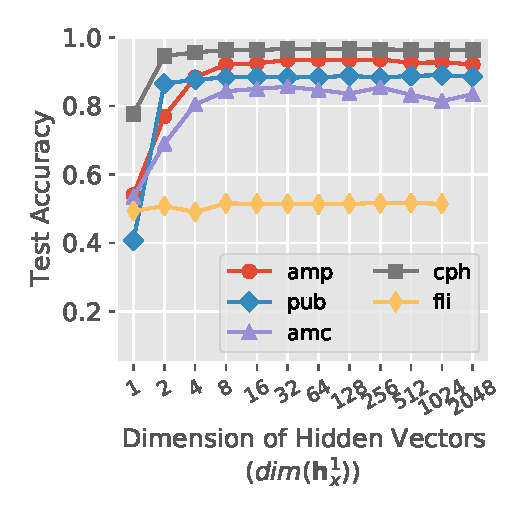
\includegraphics[width=0.3\columnwidth]{figs/experiments/exp_hyperparameter_on_accuracy_gcn.pdf}}
    \subfloat[GGNN]{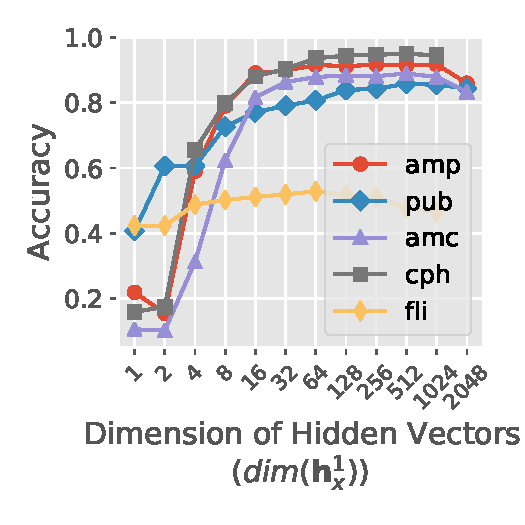
\includegraphics[width=0.3\columnwidth]{figs/experiments/exp_hyperparameter_on_accuracy_ggnn.pdf}}\\
    \subfloat[GAT]{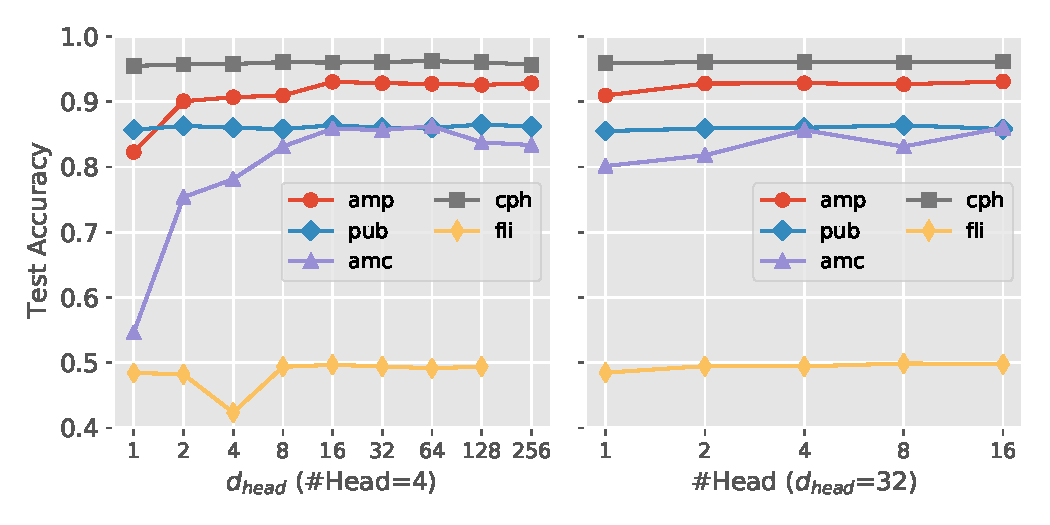
\includegraphics[width=0.6\columnwidth]{figs/experiments/exp_hyperparameter_on_accuracy_gat.pdf}}\\
    \subfloat[GaAN]{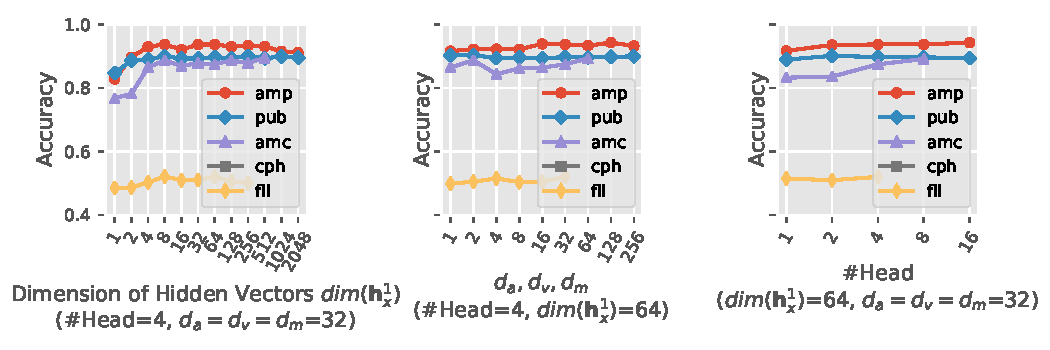
\includegraphics[width=0.9\columnwidth]{figs/experiments/exp_hyperparameter_on_accuracy_gaan.pdf}}
    \caption{Effects of hyper-parameters on the accuracy of the typical GNNs.}
    \label{fig:exp_hyperparameter_accuracy}
\end{figure}

\figurename~\ref{fig:exp_hyperparameter_on_accuracy_alg_contrast} further compares the best accuracy that every GNN achieved on different datasets.
%
The best accuracy of the four GNNs was very close.
%
%
It was also close to the accuracy reported in \cite{shchur2018_pitfall_of_gnn, zeng2020_graphsaint}.
%
The results indicated that there was no clear winner.
%
The relative accuracy between GNNs varied greatly with different datasets.
%
GaAN achieved the highest accuracy in three out of five datasets.
%
GCN achieved the highest or second-highest accuracy in three out of five datasets, though its model was simplest.
%
Simple GNN models (such as GCN) could still achieve good accuracy with proper hyper-parameter settings.

\begin{figure}[H]
    \centering
    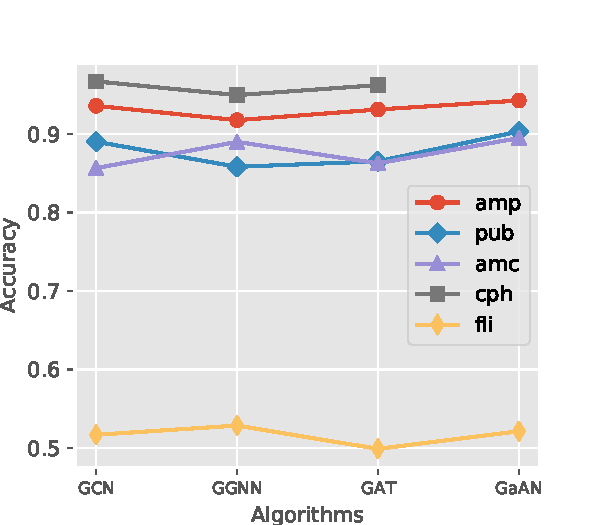
\includegraphics[width=3in]{figs/experiments/exp_hyperparameter_on_accuracy_alg_contrast.pdf}
    \caption{Best accuracy that each GNN achieved on different datasets.}
    \label{fig:exp_hyperparameter_on_accuracy_alg_contrast}
\end{figure}

\paragraph{Summary}

The complexity analysis in \tablename~\ref{tab:gnn_overview_edge} and \tablename~\ref{tab:gnn_overview_vertex} was valid for both training and inference.
%
Fixing other hyper-parameters, each hyper-parameter itself affected the training/inference time and the memory usage of a GNN layer \emph{in a linear way}.
%
Algorithm engineers could adjust hyper-parameters according to the complexity analysis to avoid explosive growth in training/inference time and memory usage.
%
The accuracy of GNNs was much more sensitive to the dimensions of hidden vectors/heads than the other hyper-parameters.
%
The relative accuracy between GNNs varied greatly with different datasets.
%
Simple GNN models (such as GCN) could achieve good accuracy with proper hyper-parameter settings.

\subsection{Time Breakdown Analysis}
\label{sec:time_breakdown_analysis}

To find out which stage/step dominated the training/inference time, we decomposed the training/inference time and analyzed performance bottlenecks level by level.
%
We first analyzed the training time in Section~\ref{sec:time_breakdown_analysis_layer_level} to Section~\ref{sec:time_breakdown_analysis_operator_level}.
%
The similarities and differences between training and inference were analyzed in Section~\ref{sec:time_breakdown_analysis_inference}.

\subsubsection{Layer Level}
\label{sec:time_breakdown_analysis_layer_level}

\figurename~\ref{fig:exp_vertex_edge_cal_proportion} decomposes the training time of a GNN on the layer level.
%
The training time of each layer was the summation of the time in the forward, backward, and evaluation phases.
%
In GCN, GAT, and GaAN, the time spent on the layer 0 was much larger than the layer 1.
%
In those GNNs, the dimensions of the input/output hidden vectors in the layer 0 were much larger than the dimensions in the layer 1: $d^0_{in}=dim(\boldsymbol{v}_x)$, $d^0_{out}=d^1_{in}=64$, $d^1_{out}=\#Class$, and $dim(\boldsymbol{v}_x) \gg \#Class$.
%
For GaAN, since it required the dimensions of the input/output hidden vectors must be the same, the hyper-parameters were set to $d^0_{in}=d^0_{out}=d^1_{in}=d^1_{out}=64$ and the training time of both layers was close.

\begin{figure}[H]
    \centering
    \subfloat[GCN\label{fig:exp_vertex_edge_cal_proportion_gcn}]{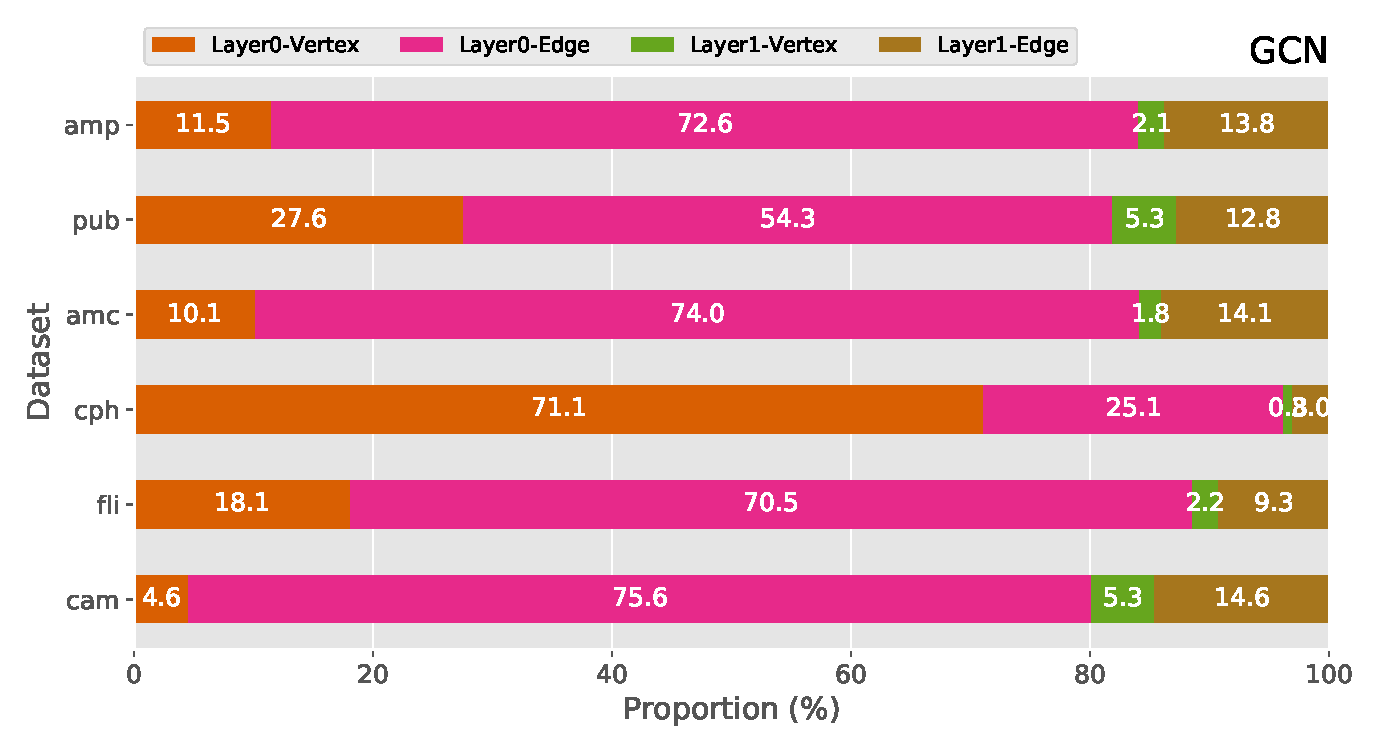
\includegraphics[height=4.6cm]{figs/experiments/exp_layer_time_proportion_gcn.pdf}}
    \subfloat[GGNN]{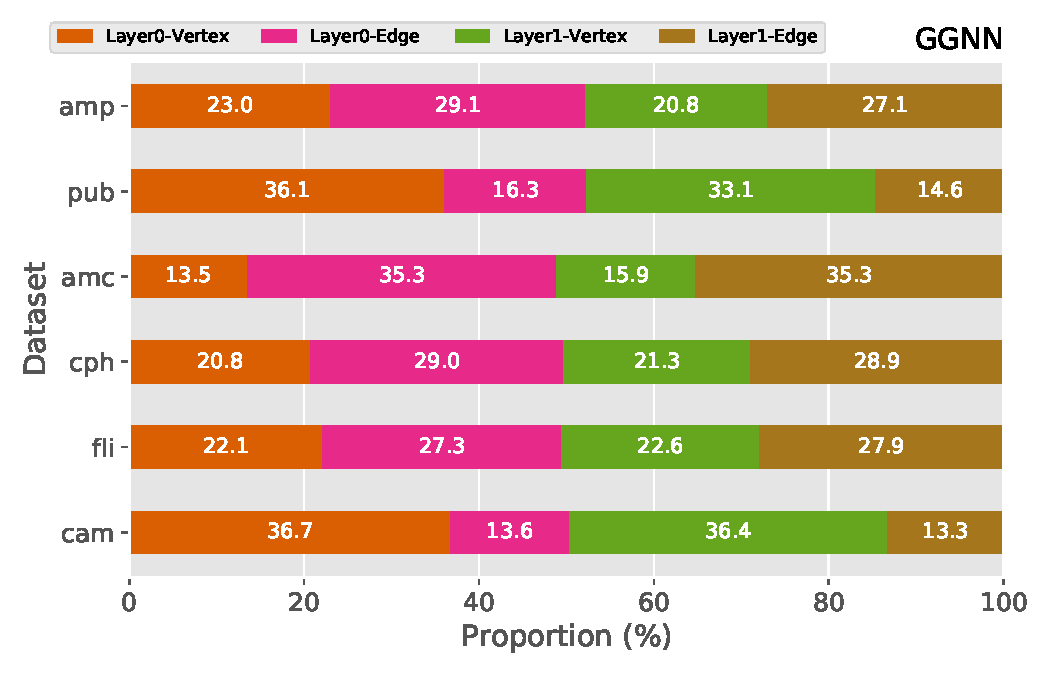
\includegraphics[height=4.6cm]{figs/experiments/exp_layer_time_proportion_ggnn.pdf}}\\
    \subfloat[GAT]{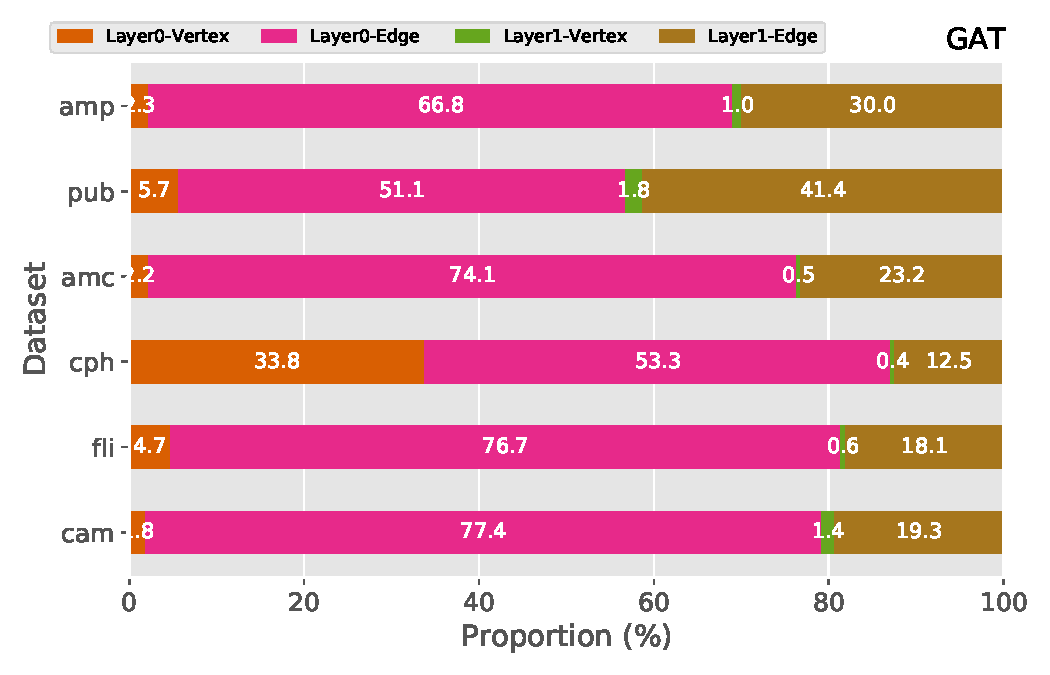
\includegraphics[height=4.6cm]{figs/experiments/exp_layer_time_proportion_gat.pdf}}
    \subfloat[GaAN]{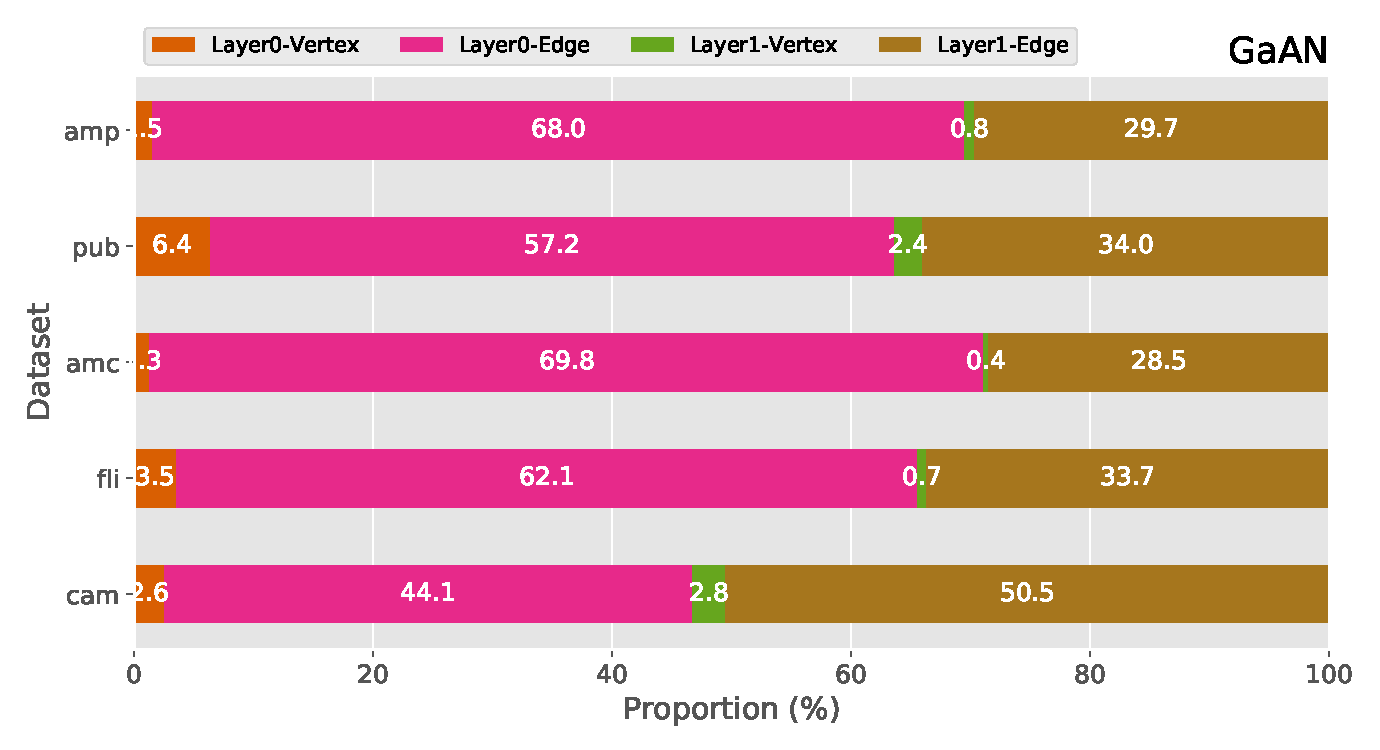
\includegraphics[height=4.6cm]{figs/experiments/exp_layer_time_proportion_gaan.pdf}}
    \caption{Training time breakdown on the layer level. The training time of each layer included the time spent on the forward, backward, and evaluation phases. Each layer was further decomposed into the vertex and the edge calculation stages.}
    \label{fig:exp_vertex_edge_cal_proportion}
\end{figure}

Each GNN layer was further divided into the vertex and edge calculation stages.
%
In \figurename~\ref{fig:exp_vertex_edge_cal_proportion}, GCN spent most of the training time on the edge calculation stage on most datasets.
%
A special case was the \texttt{cph} dataset.
%
The dimension of the input feature vectors was very high in \texttt{cph}, making the vertex calculation stage of the GCN Layer 0 spend considerable time.
%
GGNN also spent the majority of its training time on the edge calculation stage, but the high time complexity of its vertex updating function $\gamma^l$ made the proportion of the vertex calculation in the total training time much higher than the other GNNs.
%
For GAT and GaAN, due to their high edge calculation complexity, the edge calculation stage was the dominant stage.

The experimental results also indicated that the average degree of the dataset affected the proportion of the edge/vertex calculation time in the total training time.
%
For GaAN, the time spent on the vertex calculation stage exceeded the edge calculation stage on the \texttt{pub} and \texttt{cam} datasets, because the average degrees of the two datasets were low, making $|\mathcal{E}|$ and $|\mathcal{V}|$ much closer.
%
To evaluate the effects of the average degree, we generated random graphs with 50,000 vertices and average degrees ranging from 2 to 100.
%
\figurename~\ref{fig:exp_avg_degree_on_vertex_edge_cal_time} shows the training time of the four GNNs under different average degrees.
%
As the average degree increased, the training time of the edge calculation stage grew \emph{linearly}.
%
For GCN, GAT, and GaAN, the edge calculation stage dominated the entire training time even when the average degrees were small.
%
Only for GGNN that had high vertex and low edge calculation complexity, the training time of the vertex calculation stage exceeded the edge calculation stage under low average degrees ($<5$).

In summary, \emph{the edge calculation stage was the most time-consuming stage in GNN training}.
%
Improving its efficiency was the key to reduce the GNN training time.

\begin{figure}[H]
    \centering
    \subfloat[GCN\label{fig:exp_avg_degree_on_vertex_edge_cal_time_gcn}]{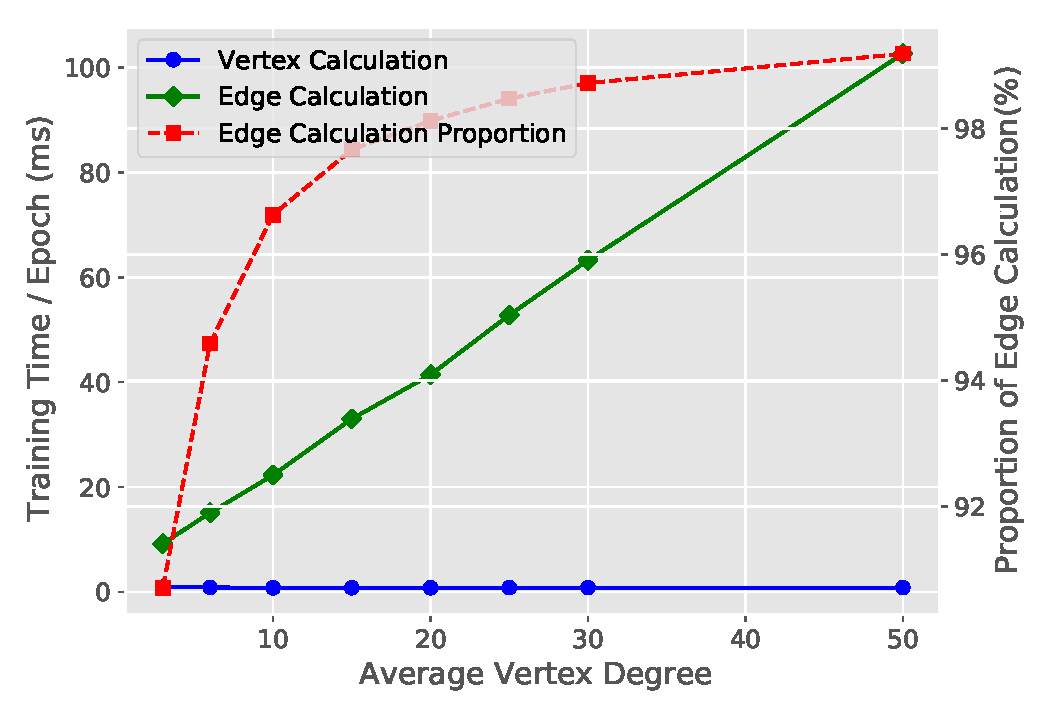
\includegraphics[height=4cm]{figs/experiments/exp_avg_degree_on_vertex_edge_cal_time_gcn.pdf}}
    \subfloat[GGNN]{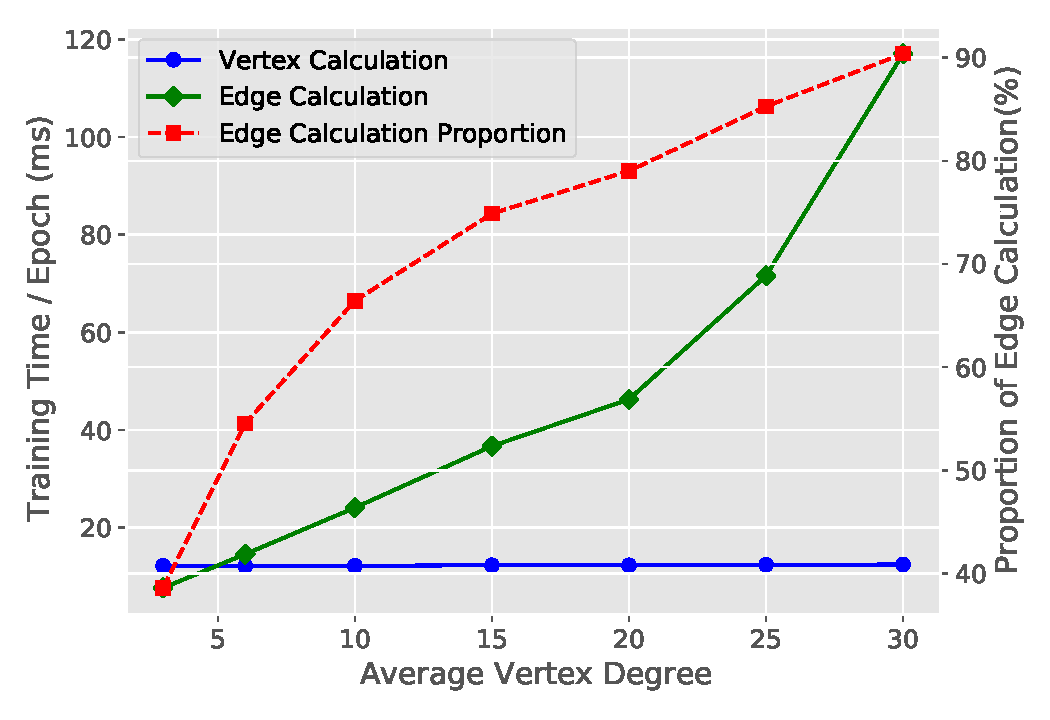
\includegraphics[height=4cm]{figs/experiments/exp_avg_degree_on_vertex_edge_cal_time_ggnn.pdf}}\\
    \subfloat[GAT]{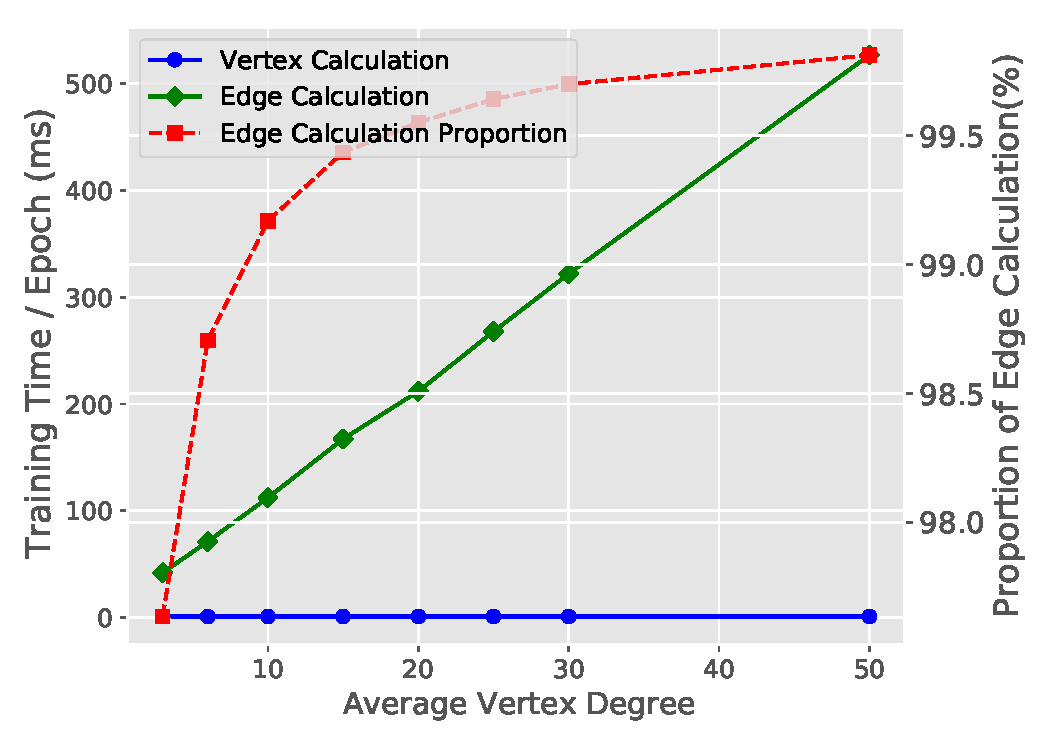
\includegraphics[height=4cm]{figs/experiments/exp_avg_degree_on_vertex_edge_cal_time_gat.pdf}}
    \subfloat[GaAN]{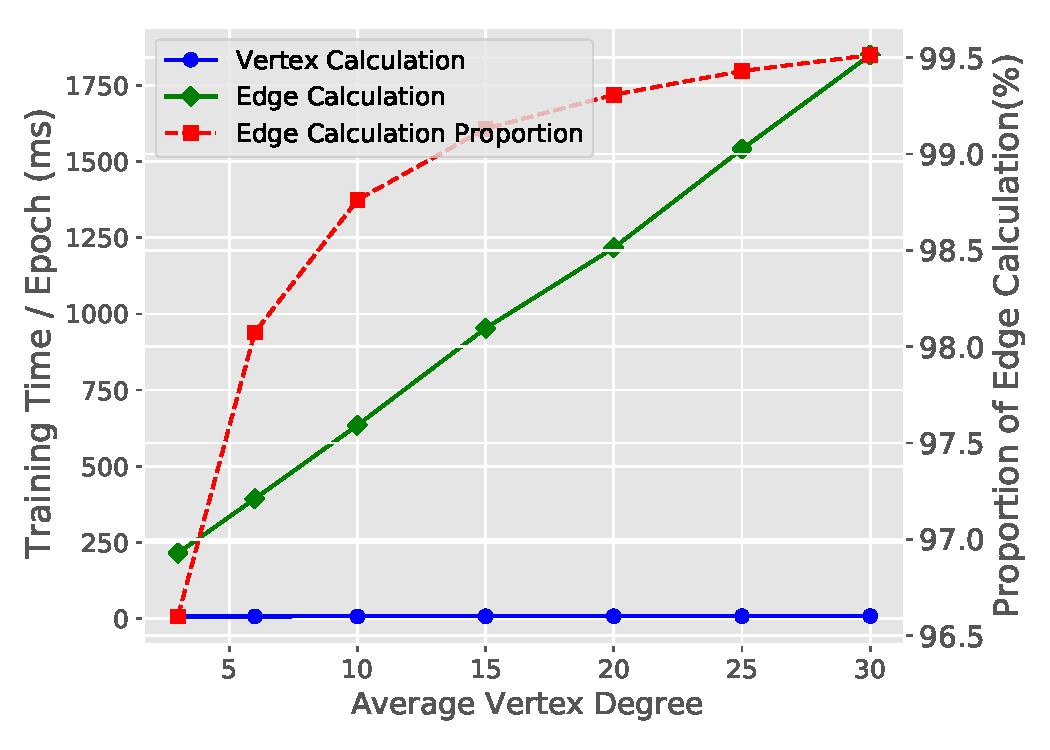
\includegraphics[height=4cm]{figs/experiments/exp_avg_degree_on_vertex_edge_cal_time_gaan.pdf}}
    \caption{Effects of average degrees on the vertex/edge calculation time. Graphs were generated with the R-MAT generator by fixing the number of vertices as 50,000. }
    \label{fig:exp_avg_degree_on_vertex_edge_cal_time}
\end{figure}

\subsubsection{Step Level in Edge Calculation}

We further investigated the most time-consuming step of the edge calculation stage.
%
In the implementation of PyG, the edge calculation stage consisted of four steps: collection, messaging, aggregation, and vector updating, as shown in \figurename~\ref{fig:steps_in_edge_calculation}.
%
The edge index was a matrix with $|\mathcal{E}|$ rows and two columns.
%
It held the edge set of the graph.
%
The two columns of the edge index stored the source and the target vertex IDs of each edge.
%
The collection step copied the hidden vectors from the previous GNN layer $\MyVec{h}^l_y$ and $\MyVec{h}^l_x$ to the both endpoints of each edge $e_{y,x}$ in the edge index, forming the parameter tensor $[\MyVec{h}^l_{y}, \MyVec{h}^l_{x}, \MyVec{e}_{y,x}]$ of the messaging function $\phi^l$.
%
This step only involved data movement.
%
The messaging step called the messaging function $\phi^l$ on all edges to get message vectors $\MyVec{m}^l_{y,x}$.
%
The aggregation step aggregated the message vectors with the same target vertex into an aggregated vector $\MyVec{s}^l_x$.
%
The vector updating step was optional.
%
It performed an additional transformation on the aggregated vectors (for example, adding the bias in GCN).

\begin{figure}[H]
    \centering
    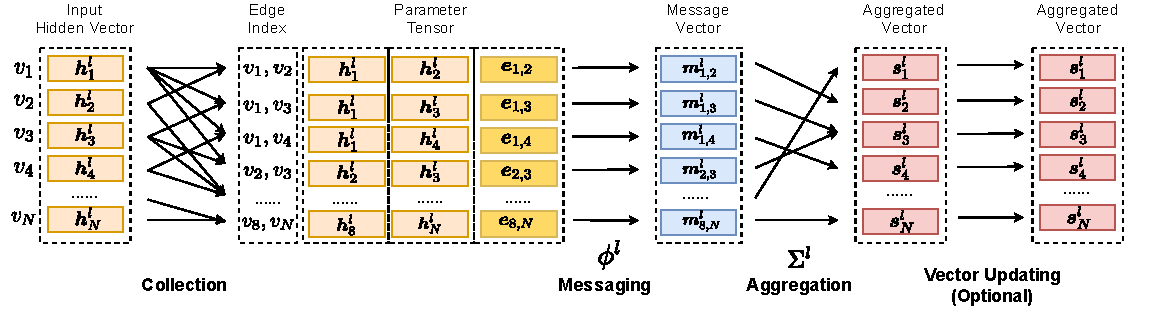
\includegraphics[width=1\columnwidth]{figs/illustration/steps_in_edge_calculation.pdf}
    \caption{Step decomposition of the edge calculation stage of the GNN layer $l$.}
    \label{fig:steps_in_edge_calculation}
\end{figure}

We decomposed the execution time of the edge calculation stage in \figurename~\ref{fig:exp_edge_calc_decomposition}.
%
In each GNN, the proportions of the four steps were rather stable, rarely affected by datasets. 
%
For GAT and GaAN with the high edge calculation complexity, the messaging step consumed most of the training time. 
%
For GCN and GGNN with the low edge complexity, the proportions of the steps were close. 
%
Since the messaging function $\phi^l$ of GGNN used the pre-computed $\MyVec{\hat{h}}^l_y$ as the message vector directly, the time spent on the messaging step of GGNN was negligible.
%
Although the collecting step did not conduct any computation and only involved data movement, it occupied noticeable execution time in the four GNNs.

The results indicate that \emph{the performance bottlenecks of the edge calculation stage depend on the complexity of the messaging function $\phi$}.
%
When the time complexity of $\phi$ was high, the messaging step was the performance bottleneck.
%
Optimizing the implementation of $\phi$ could significantly reduce training time.
%
Otherwise, the collection and the aggregation steps were performance bottlenecks.
%
Improving the efficiency of the two steps could benefit all GNNs.

\begin{figure}[H]
    \centering
    \subfloat[GCN\label{fig:exp_edge_calc_decomposition_gcn}]{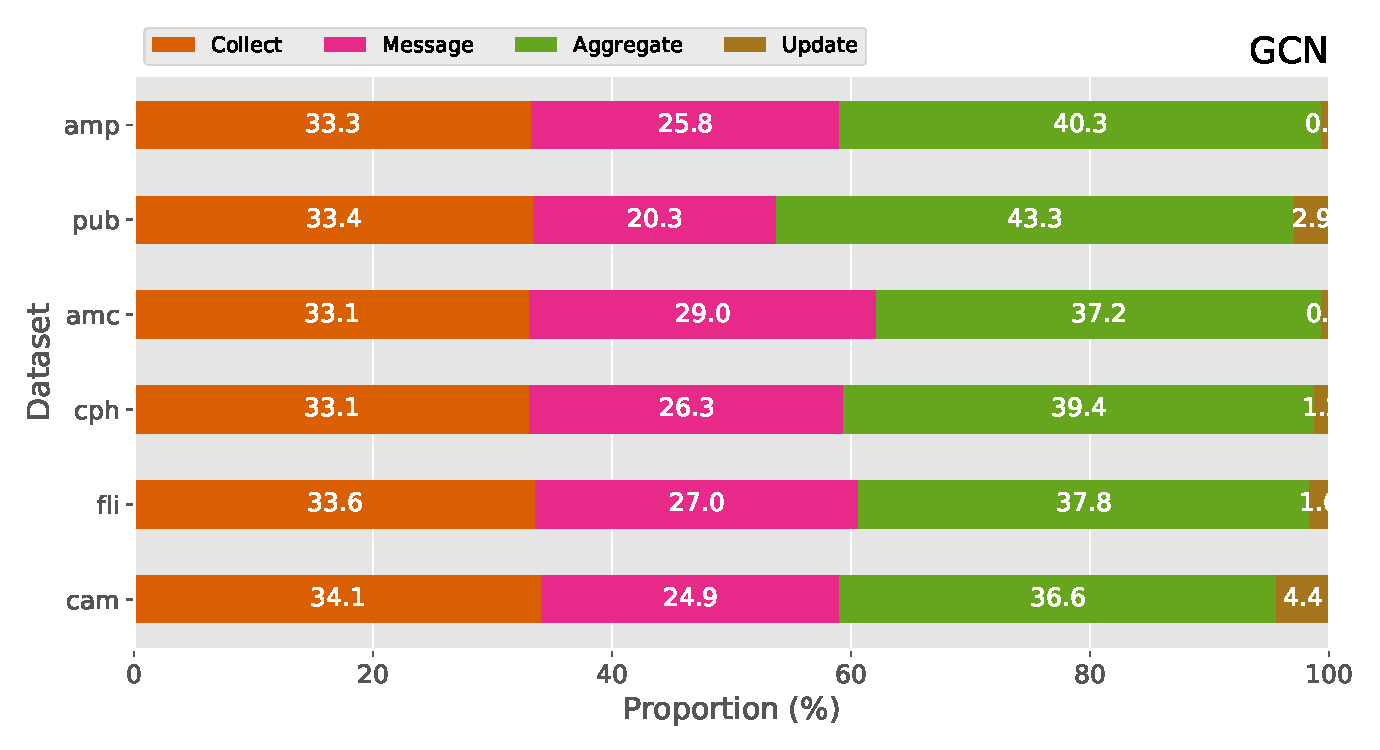
\includegraphics[width=0.5\columnwidth]{figs/experiments/exp_edge_calc_decomposition_gcn.pdf}}
    \subfloat[GGNN]{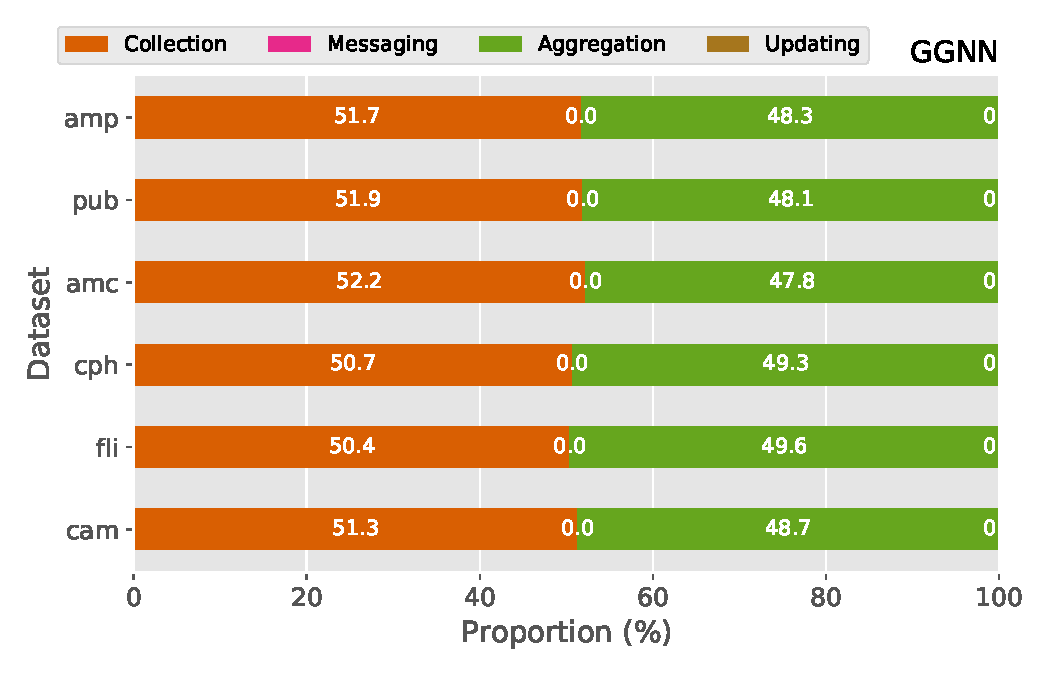
\includegraphics[width=0.5\columnwidth]{figs/experiments/exp_edge_calc_decomposition_ggnn.pdf}}\\
    \subfloat[GAT]{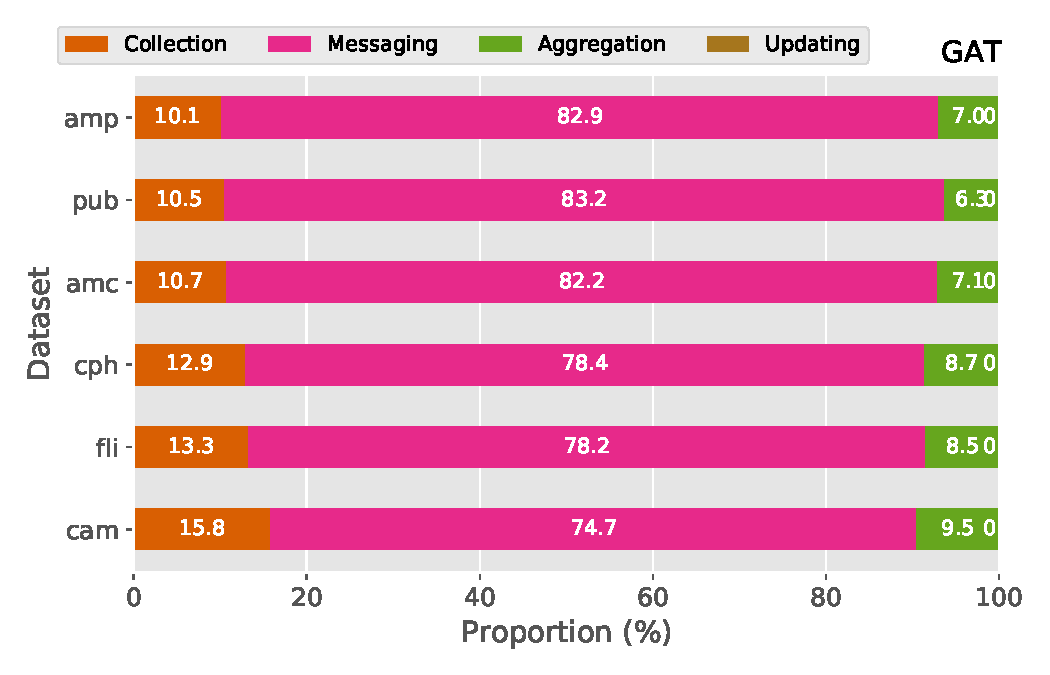
\includegraphics[width=0.5\columnwidth]{figs/experiments/exp_edge_calc_decomposition_gat.pdf}}
    \subfloat[GaAN]{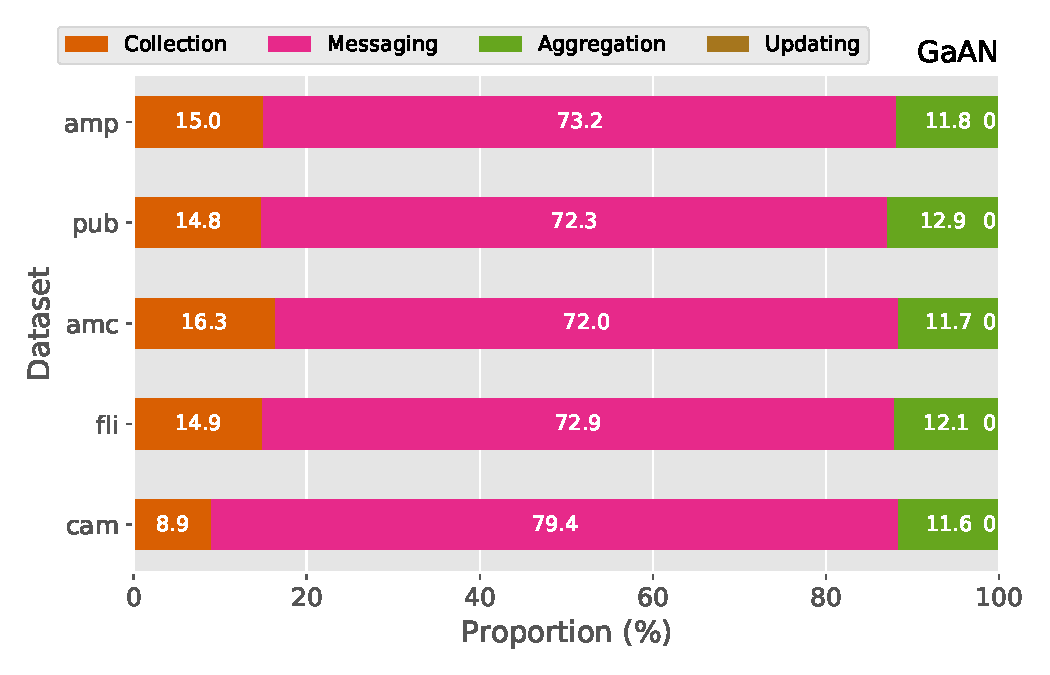
\includegraphics[width=0.5\columnwidth]{figs/experiments/exp_edge_calc_decomposition_gaan.pdf}}
    \caption{Training time breakdown of the edge calculation stage.}
    \label{fig:exp_edge_calc_decomposition}
\end{figure}

\subsubsection{Operator Level}
\label{sec:time_breakdown_analysis_operator_level}

The functions $\phi$, $\Sigma$ and $\gamma$ in the edge and vertex calculation stages were made up of a series of basic operators implemented on the GPU side, such as the matrix multiplication \texttt{mm}, the elementwise multiplication \texttt{mul} and the index-based selection \texttt{index\_select}.
%
\figurename~\ref{fig:exp_top_basic_ops} shows the top-5 time-consuming basic operators of training each GNN, averaged over all datasets.

\begin{figure}[H]
    \centering
    \subfloat[GCN]{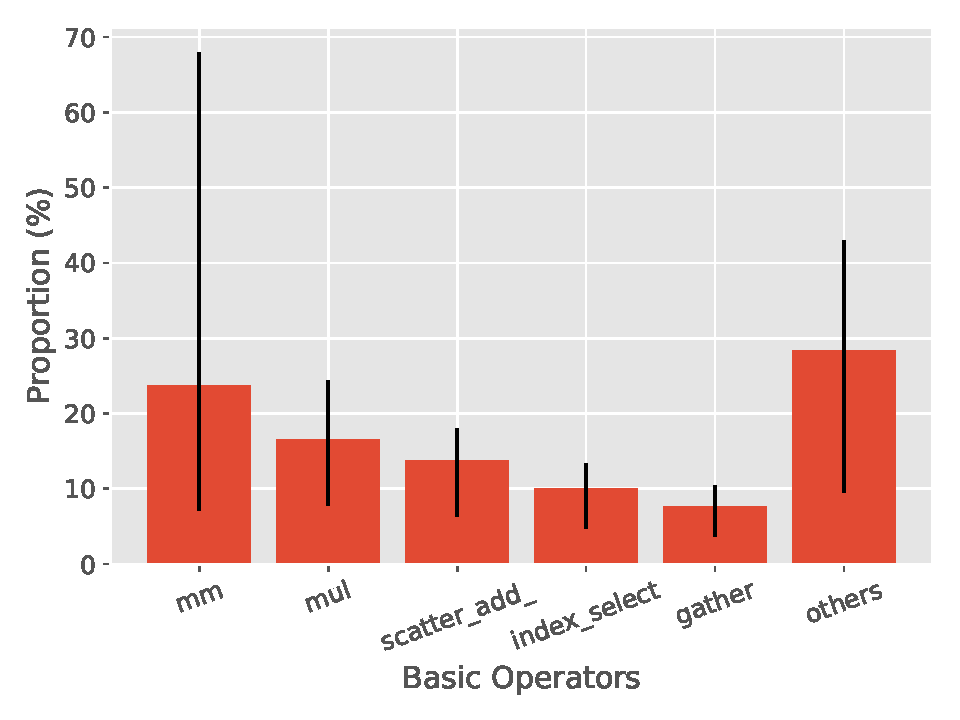
\includegraphics[height=4cm]{figs/experiments/exp_top_basic_ops_gcn.pdf}}
    \subfloat[GGNN]{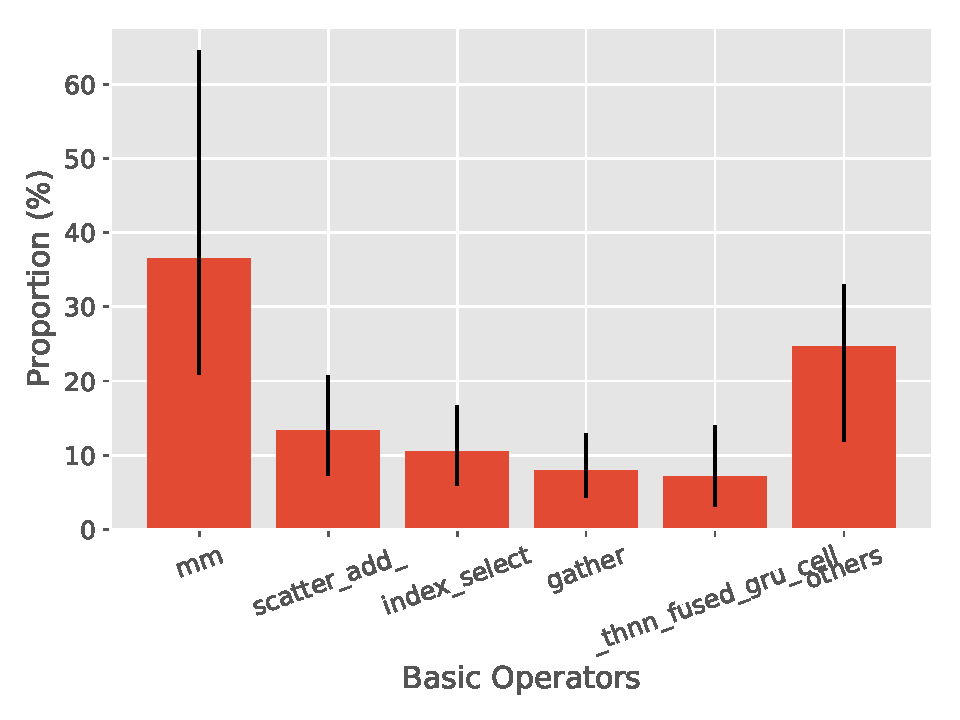
\includegraphics[height=4cm]{figs/experiments/exp_top_basic_ops_ggnn.pdf}}\\
    \subfloat[GAT\label{fig:exp_top_basic_ops_gat}]{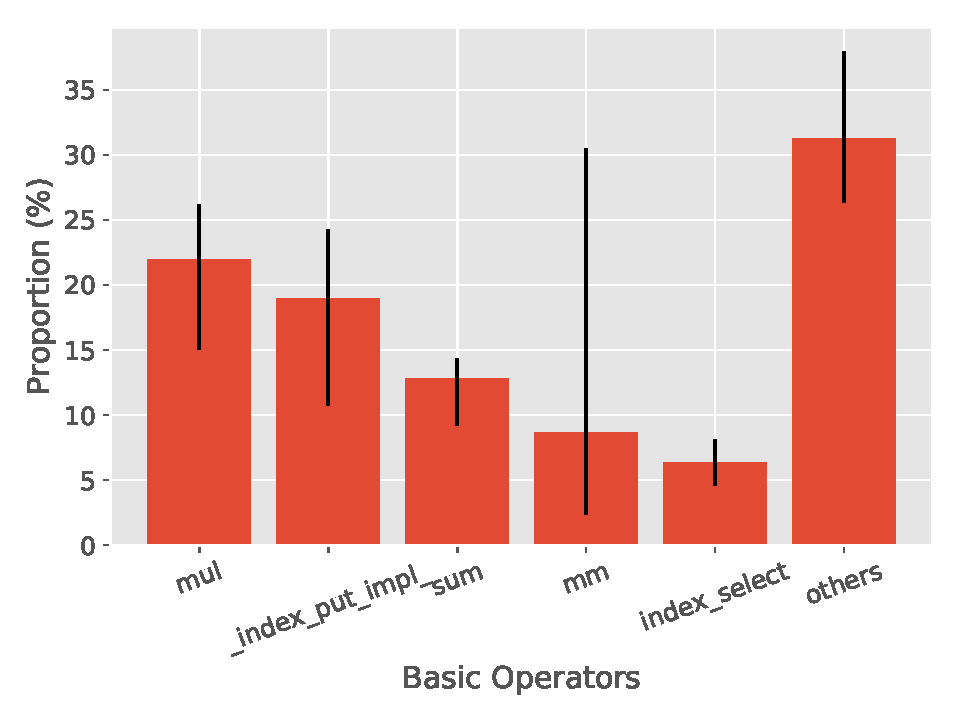
\includegraphics[height=4cm]{figs/experiments/exp_top_basic_ops_gat.pdf}}
    \subfloat[GaAN]{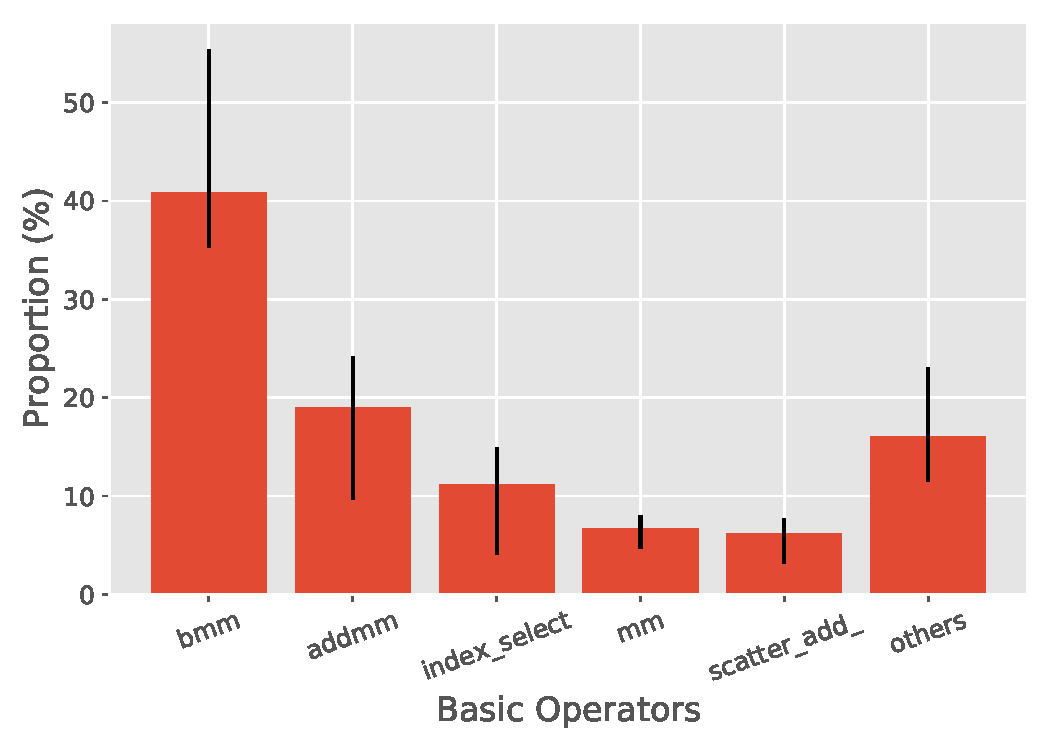
\includegraphics[height=4cm]{figs/experiments/exp_top_basic_ops_gaan.pdf}}
    \caption{Top 5 time-consuming basic operators in training. The time proportion of each basic operator was averaged over all datasets with the error bar indicating the maximum and the minimum.}
    \label{fig:exp_top_basic_ops}
\end{figure}

\paragraph{GCN}
%
The most time-consuming basic operator was the matrix multiplication \texttt{mm} used in the vertex updating function $\gamma$.
%
The elementwise multiplication \texttt{mul} used in the messaging function $\phi$ was also time-consuming.
%
The other three operators were used in the edge calculation stage: \texttt{scatter\_add\_} for the aggregation step in the forward phase, \texttt{gather} for the aggregation step in the backward phase, and \texttt{index\_select} for the collection step.
%
For GCN, the basic operators related to the edge calculation stage consumed the majority of the training time.

\paragraph{GGNN}
%
The top basic operator was \texttt{mm} used in the vertex updating function $\gamma$.
%
Due to its high time complexity, the proportion of \texttt{mm} was much higher than the other operators.
%
The \texttt{thnn\_fused\_gru\_cell} operator was used in both the forward and backward phases of $\gamma$.
%
The other three operators were used in the edge calculation stage.

\paragraph{GAT}
%
All the top basic operators except for \texttt{mm} were related to the edge calculation stage.
%
The \texttt{mm} operator was used in the vertex updating function $\gamma$.

\paragraph{GaAN}
%
The top basic operator was \texttt{bmm} used in the messaging function $\phi$.
%
The \texttt{addmm} operator and the \texttt{mm} operator were used in both the vertex and the edge calculation stages, where the edge calculation stage was dominant.

The most time-consuming operators in the four GNNs were the matrix multiplication \texttt{mm} and the elementwise multiplication \texttt{mul}, \emph{making GNN training suitable for GPUs}.
%
Although the aggregation step in the edge calculation stage was relatively simple (like sum and mean), the related operators--\texttt{scatter\_add} and \texttt{gather}--still consumed a certain amount of the time.
%
The two operators had to synchronize between hardware threads to avoid updating the same aggregated vector at the same time.
%
They also conducted non-regular memory access with the access pattern determined by the edge set dynamically.
%
For GPUs, they were less efficient than \texttt{mm}.
%
The index-based selection operator \texttt{index\_select} used in the collection step consumed about 10\% of the training time in all GNNs.
%
Improving the efficiency of \texttt{scatter\_add}/\texttt{gather}/\texttt{index\_select} could benefit all kinds of GNNs.


\subsubsection{Comparing Inference and Training}
\label{sec:time_breakdown_analysis_inference}

%
We found that the performance characteristics of GNN inference were highly similar to training on the \emph{layer} level and the \emph{step} level.
%
Taking GCN as an example, \figurename~\ref{fig:inference_analysis_of_gcn} shows the time breakdowns of GCN inference on the \emph{layer} level and \emph{step} level of the edge calculation.
%
By cross-comparing \figurename~\ref{fig:exp_vertex_edge_cal_proportion_gcn} with \figurename~\ref{fig:inference_analysis_of_gcn_layer_level}, 
\figurename~\ref{fig:exp_avg_degree_on_vertex_edge_cal_time_gcn} with \figurename~\ref{fig:inference_analysis_of_gcn_avg_degree}, and \figurename~\ref{fig:exp_edge_calc_decomposition_gcn} with \figurename~\ref{fig:inference_analysis_of_gcn_edge_level}, the time breakdowns of training and inference were very similar.
%
For the other GNNs, we observed similar phenomena.

\begin{figure}[H]
    \centering
    \subfloat[Layer level\label{fig:inference_analysis_of_gcn_layer_level}]{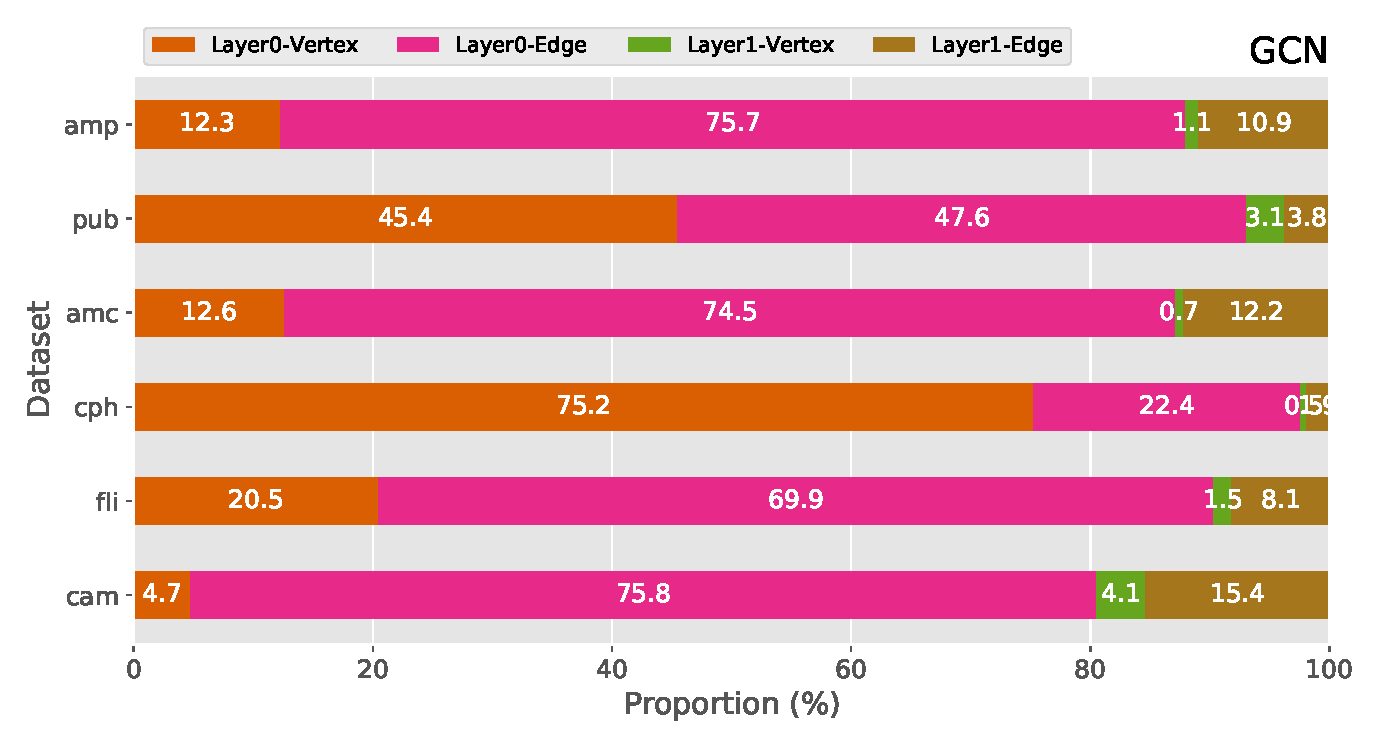
\includegraphics[width=0.5\columnwidth]{figs/experiments/exp_inference_full_layer_time_proportion_gcn.pdf}}
    \subfloat[Effects of average degrees\label{fig:inference_analysis_of_gcn_avg_degree}]{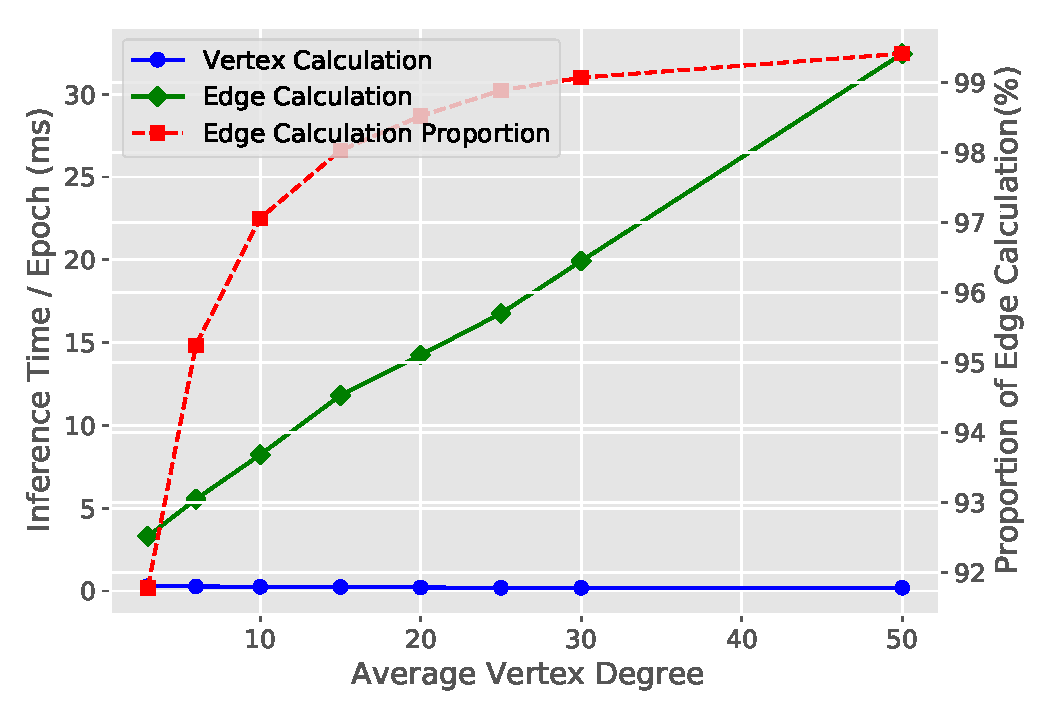
\includegraphics[width=0.4\columnwidth]{figs/experiments/exp_inference_full_avg_degree_on_vertex_edge_cal_time_gcn.pdf}}\\
    \subfloat[Step level of the edge calculation stage\label{fig:inference_analysis_of_gcn_edge_level}]{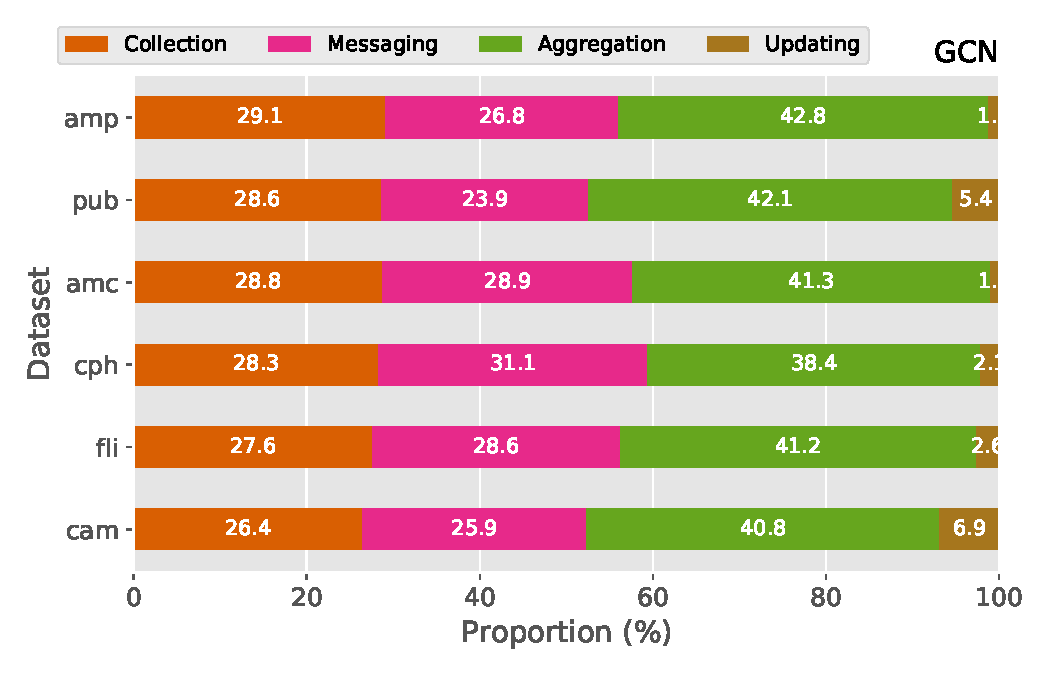
\includegraphics[width=0.5\columnwidth]{figs/experiments/exp_inference_full_edge_calc_decomposition_gcn.pdf}}
    \caption{Time breakdowns of GCN inference.}
    \label{fig:inference_analysis_of_gcn}
\end{figure}

The main differences between training and inference were reflected in two aspects: the wall-clock time and the top time-consuming basic operators.
%
The inference time was much less than the training time.
%
Figure~\ref{fig:compare_wall_clock_time_of_training_and_inference} compares the wall-clock time of training and inference on the \texttt{amp}, \texttt{amc}, and \texttt{fli} datasets.
%
The results on the other datasets were similar.
%
Since the inference only conducted the forward propagation from the input layer to the prediction layer, the time of inference was very close to the time of the forward phase in training.
%
The inference time was 34\% (GCN), 32\% (GGNN), 25\% (GAT), and 32\% (GaAN) of the training time, averaged over all datasets.

\begin{figure}[H]
    \centering
    \subfloat[\texttt{amc}]{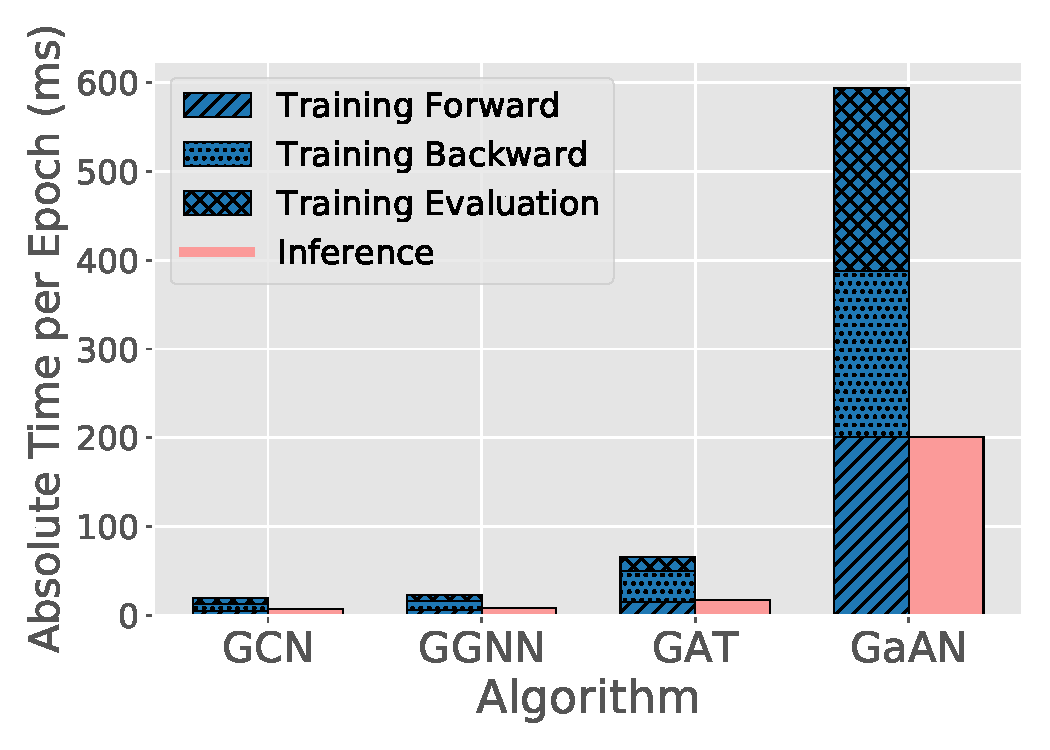
\includegraphics[width=0.3\columnwidth]{figs/experiments/exp_time_comparison_between_training_inference_amazon-computers.pdf}}
    \subfloat[\texttt{amp}]{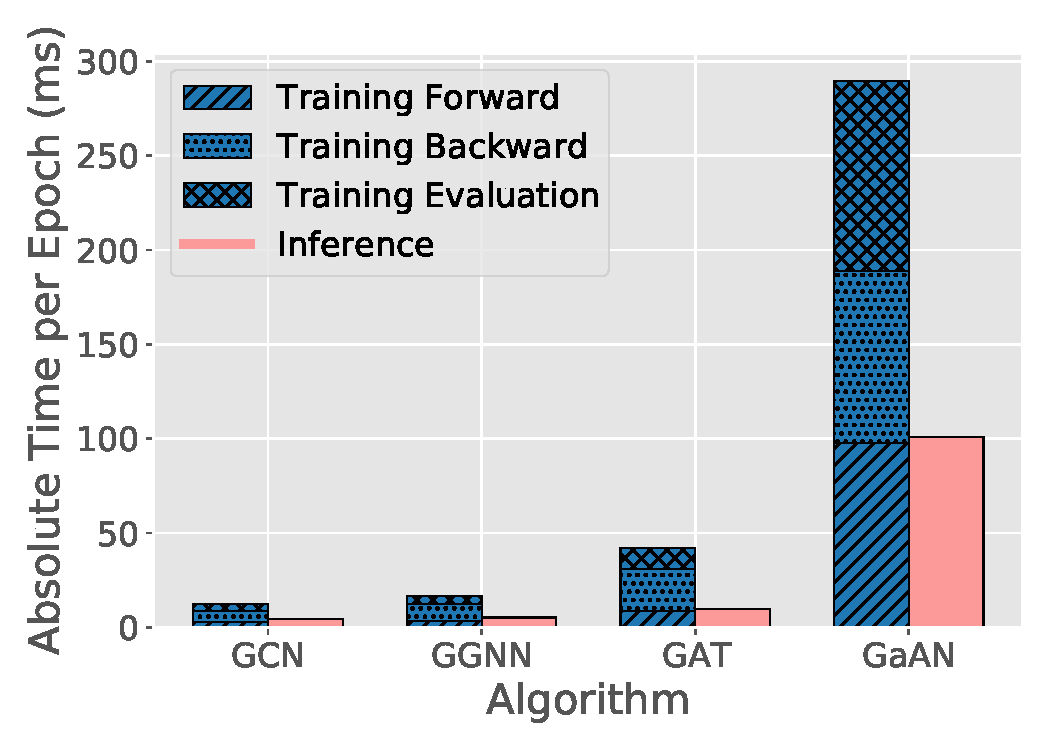
\includegraphics[width=0.3\columnwidth]{figs/experiments/exp_time_comparison_between_training_inference_amazon-photo.pdf}}
    \subfloat[\texttt{fli}]{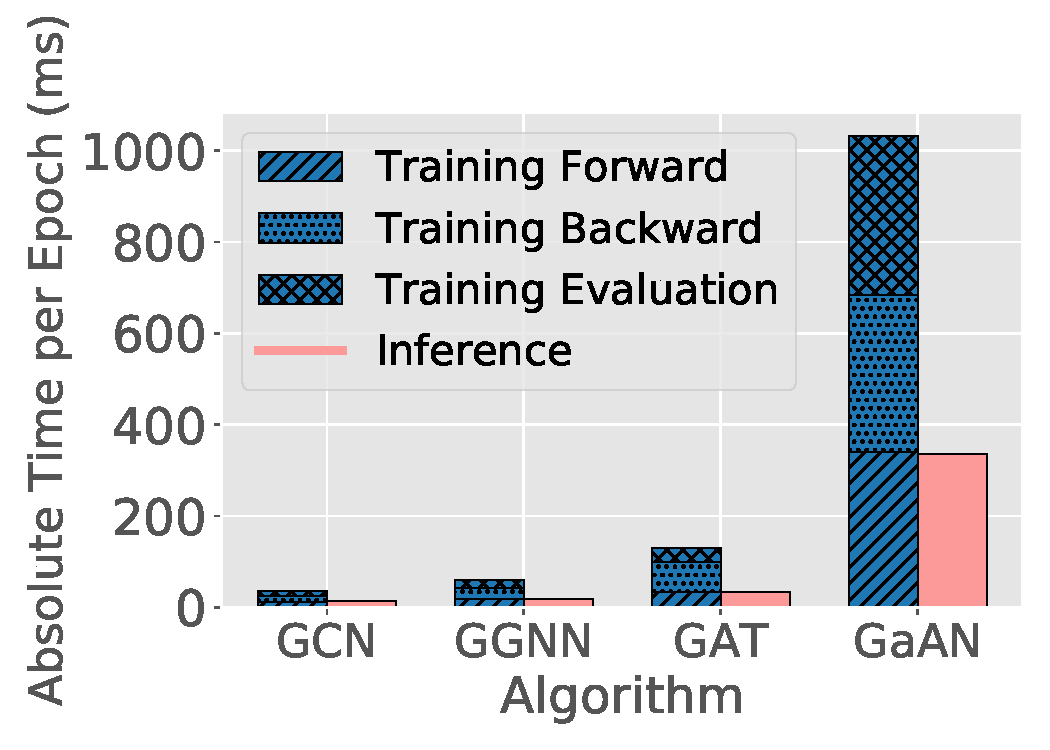
\includegraphics[width=0.3\columnwidth]{figs/experiments/exp_time_comparison_between_training_inference_flickr.pdf}}
    \caption{Wall-clock inference time on different datasets.}
    \label{fig:compare_wall_clock_time_of_training_and_inference}
\end{figure}

The top time-consuming basic operators of training and inference also showed a certain degree of difference.
%
Some of the top time-consuming operators during training were replaced by new operators in inference.
%
Figure~\ref{fig:exp_inference_top_basic_ops} shows the top 5 time-consuming basic operators in inference.
%
For GCN, the \texttt{index} operator used in the prediction layer became the new top 5 time-consuming operators, replacing the \texttt{gather} operator used in the backward phase in training.
%
%    The basic operators related to the edge calculation (\texttt{scatter\_add}, \texttt{index\_select}, and \texttt{mul}) still consumed the majority of the inference time.
%
For GGNN, \texttt{index} operator in the prediction layer also became a time-consuming basic operators.
%
%    Due to the high time complexity of the vertex updating function $\gamma$ in GGNN, the basic operators related to the vertex calculation stage (\texttt{mm} and \texttt{thnn\_fused\_gru\_cell}) still consumed near half of the inference time.
%
For GAT, the \texttt{input\_put\_impl} operator (used in the backward phase) in Figure~\ref{fig:exp_top_basic_ops_gat} was replaced by the \texttt{scatter\_add} operator used in the forward edge calculation in Figure~\ref{fig:exp_inference_top_basic_ops_gat}.
%
%    The \texttt{scatter\_add} operator was related to the edge calculation step.
%
For GaAN, the \texttt{mm} operator was replaced by the \texttt{cat} operator used in the vertex updating function.

Although some specific time-consuming operators were different, the performance bottlenecks on the operator level were the same for training and inference.
%
The matrix multiplication \texttt{mm} and the element-wise multiplication \texttt{mul} operators were still time-consuming for inference, making GNN inference also {suitable for GPUs}.
%
The basic operators related to the collection and aggregation steps in the edge calculation still consumed non-trivial time in inference.

\begin{figure}[H]
    \centering
    \subfloat[GCN]{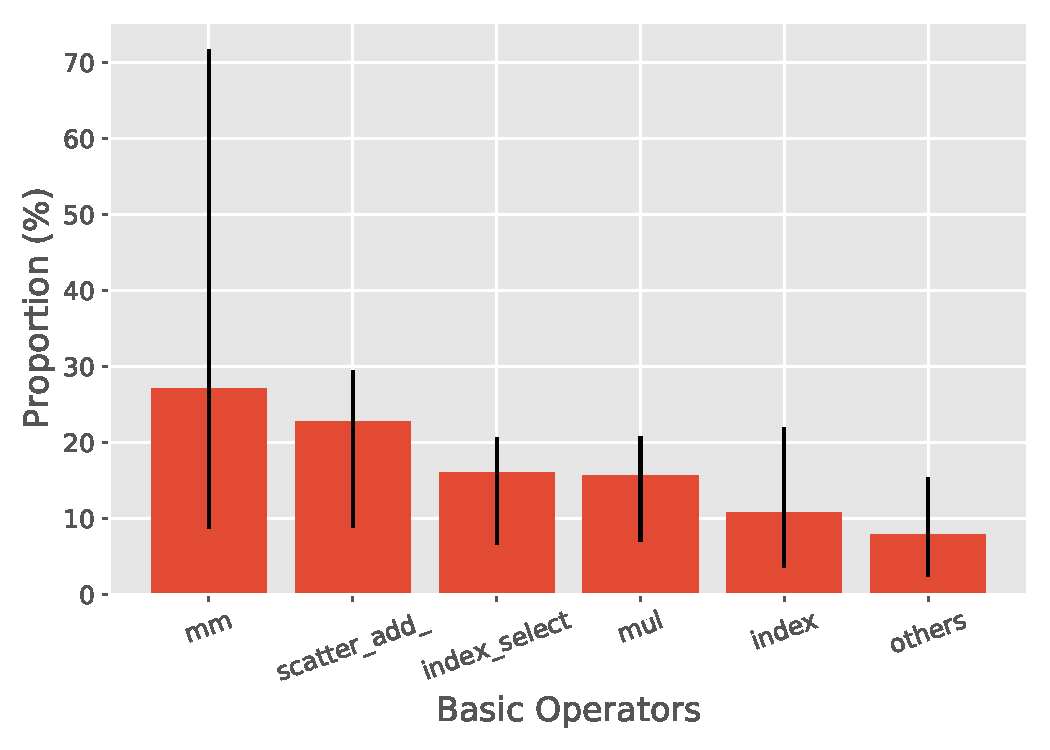
\includegraphics[height=4cm]{figs/experiments/exp_inference_full_top_basic_ops_gcn.pdf}}
    \subfloat[GGNN]{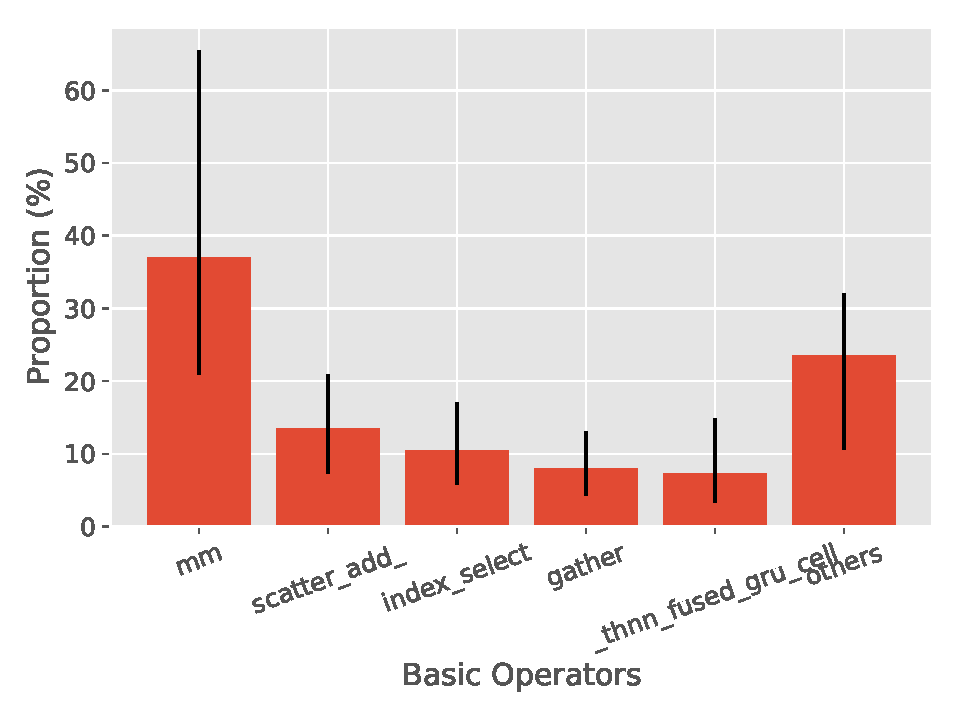
\includegraphics[height=4cm]{figs/experiments/exp_inference_full_top_basic_ops_ggnn.pdf}}\\
    \subfloat[GAT\label{fig:exp_inference_top_basic_ops_gat}]{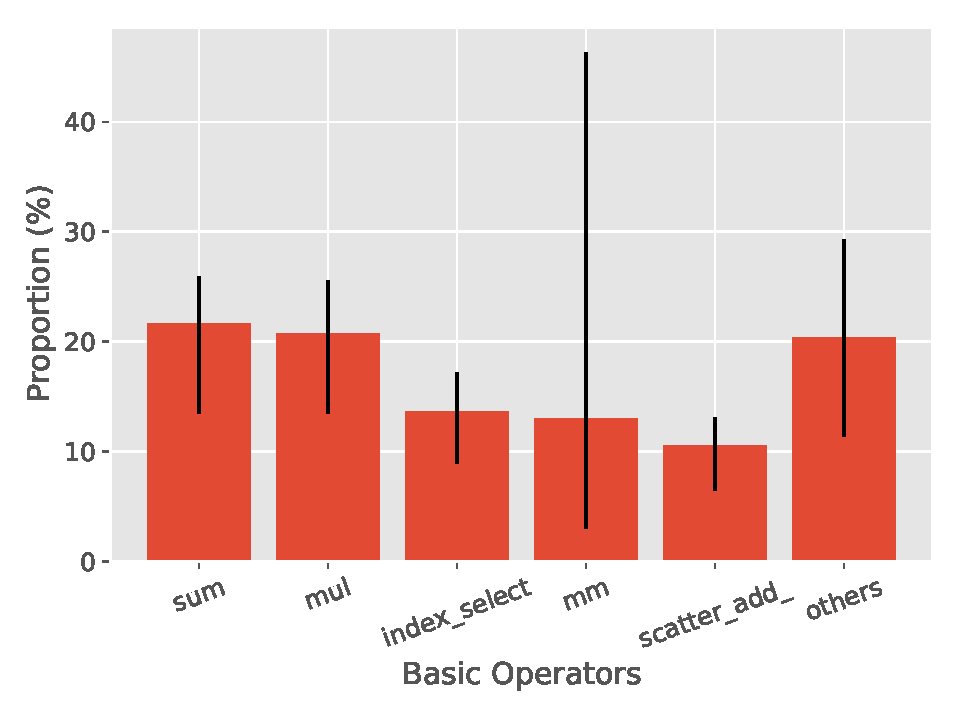
\includegraphics[height=4cm]{figs/experiments/exp_inference_full_top_basic_ops_gat.pdf}}
    \subfloat[GaAN]{\includegraphics[height=4cm]{figs/experiments/exp_inference_full_top_basic_ops_gaan.pdf}}
    \caption{Top 5 time-consuming basic operators in inference. The time proportion of each basic operator was averaged over all datasets with the error bar indicating the maximum and the minimum.}
    \label{fig:exp_inference_top_basic_ops}
\end{figure}

\paragraph{Summary of Time Breakdown Analysis}

The GNN training/inference was suitable for GPUs.
%
{The edge calculation stage was the main performance bottleneck in most cases}, except for processing GNNs with high vertex calculation complexity on low-average-degree graphs.
%
The performance bottlenecks in the edge calculation stage depended on the time complexity of the messaging function $\phi$.
%
If the time complexity of $\phi$ was {high}, {$\phi$} dominated the training/inference time of the edge calculation stage.
%
Optimizations should focus on improving its efficiency.
%
Otherwise, the {collection step} and the {aggregation step} dominated the training/inference time.
%
The collection step suffered from lots of data movement.
%
The aggregation step suffered from data synchronization and non-regular data access.

\subsection{Memory Usage Analysis}
\label{sec:memory_usage_analysis}

\paragraph{Training}

During the GNN training, we stored all data (including datasets and intermediate results) in the on-chip memory of the GPU.
%
Compared with the main memory on the host side (90 GB), the capacity of the GPU memory (16 GB) was very limited.
%
\emph{The GPU memory capacity limited the scales of the graphs that it could handle}.
%
For example, GaAN was unable to train on the \texttt{cph} dataset due to the out of memory exception.

\figurename~\ref{fig:exp_memory_usage_stage_amp} shows the peak memory usage of each phase during the GNN training on the \texttt{amp} dataset.
%
The trends on the other datasets were similar.
%
\emph{The GNN training achieved its peak memory usage in the forward and the backward phases}.
%
The forward phase generated lots of intermediate results.
%
Some key intermediate results were cached for the gradient calculation in the backward phase, increasing memory usage.
%
For example, \figurename~\ref{fig:ggnn_vertex_func_computation_graph} shows the computation graph of the vertex updating function $\gamma^l$ of GGNN.
%
Each operator in the computation graph generated an intermediate tensor.
%
Some key intermediate tensors were cached.
%
The cached tensors were the main source of memory usage in the loss phase.
%
By the end of the backward phase, the cached tensors were released.
%
Since the evaluation phase did not have to calculate the gradients, it did not cache intermediate tensors.
%
Its memory usage declined sharply.

\begin{figure}[H]
    \centering
    \includegraphics[height=5cm]{figs/experiments/exp_memory_usage_stage_amp.pdf}
    \caption{Memory usage of each phase during the GNN training. Dataset: \texttt{amp}.}
    \label{fig:exp_memory_usage_stage_amp}
\end{figure}

\begin{figure}[H]
    \centering
    \includegraphics[width=0.7\columnwidth]{figs/illustration/ggnn_vertex_func_computation_graph.pdf}
    \caption{Computation graph of the vertex updating function $\gamma$ of GGNN.}
    \label{fig:ggnn_vertex_func_computation_graph}
\end{figure}

The peak memory usage during the GNN training far exceeded the size of the dataset itself.
%
We defined the \emph{memory expansion ratio} (MER) as the ratio of the peak memory usage during the training to the memory usage after loading the dataset.
%
\figurename~\ref{fig:exp_memory_expansion_ratio} compares MER of different GNNs.
%
GCN had the lowest MER (up to 15.2) while GaAN had the highest MER (up to 104.6).
%
\emph{The high MERs limited the data scalability of GNNs}, making GPUs unable to handle big graphs.
%
\figurename~\ref{fig:exp_memory_expansion_ratio} also indicates that the same GNN had different MERs for different datasets.
%
Two characteristics of a dataset affected the MER: the dimension of the input feature vectors and the average degree of the graph.

\begin{figure}[H]
    \centering
    \includegraphics[width=0.5\columnwidth]{figs/experiments/exp_memory_expansion_ratio.pdf}
    \caption{Memory expansion ratios of typical GNNs.}
    \label{fig:exp_memory_expansion_ratio}
\end{figure}

To find out how the dimension of input feature vectors affected the MER, we generated random input feature vectors with different dimensions for the \texttt{cam} dataset and measured the MER in \figurename~\ref{fig:exp_memory_expension_ratio_input_feature_dimension}.
%
Under the same hyper-parameters, \emph{the MER decreased as the dimension of input feature vectors increased}.
%
When the dimension of the input feature vectors was high, the size of the dataset itself was large.
%
The size became comparable to the size of intermediate results, making MERs low.


\begin{figure}[H]
    \centering
    \includegraphics[height=5cm]{figs/experiments/exp_memory_expansion_ratio_input_feature_dimension_com-amazon.pdf}
    \caption{Memory expansion ratio under different dimensions of input feature vectors. Dataset: \texttt{cam}.}
    \label{fig:exp_memory_expension_ratio_input_feature_dimension}
\end{figure}

Average degrees also affected MERs by influencing the relative sizes of intermediate results from the edge and the vertex calculation stages.
%
Fixing the number of vertices $|\mathcal{V}|$, we generated random graphs with different average degrees.
%
\figurename~\ref{fig:exp_memory_expansion_ratio_input_graph_number_of_edges} shows how the memory usage changed according to the average degree.
%
As the average degree $\bar{d}$ increased, the peak memory usage increased \emph{linearly} with $\bar{d}$.
%
The edge calculation stage gradually dominated the memory usage and \emph{the MER converged to a stable value}.
%
The stable value was determined by the complexity of the edge calculation stage.
%
Except for GGNN, the MERs of the other GNNs increased as $\bar{d}$ increased.
%
As GGNN had high vertex calculation complexity, the MERs related to the vertex calculation stage were much higher than the edge calculation stage.
%
When the edge calculation stage dominated the memory usage, its MERs became smaller.

\begin{figure}[H]
    \centering
    \subfloat[Peak memory usage]{\includegraphics[height=4cm]{figs/experiments/exp_memory_expansion_ratio_input_graph_number_of_edges_peak_memory.pdf}}
    \subfloat[Memory expansion ratio]{\includegraphics[height=4cm]{figs/experiments/exp_memory_expansion_ratio_input_graph_number_of_edges_expansion_ratio.pdf}}
    \caption{Memory usage under different average degrees. The random graphs were generated by fixing the number of vertices at 10K and the dimension of input feature vectors at 32.}
    \label{fig:exp_memory_expansion_ratio_input_graph_number_of_edges}
\end{figure}

We also fixed the number of edges $|\mathcal{E}|$ and generated random graphs with different $|\mathcal{V}|$.
%
\figurename~\ref{fig:exp_memory_expansion_ratio_input_graph_number_of_vertices_fixed_edge} shows how the memory usage changed according to $|\mathcal{V}|$.
%
MERs of all GNNs were insensitive to $|\mathcal{V}|$, compared to $|\mathcal{E}|$.
%
Except for GGNN, the MERs of the other GNNs declined as $|\mathcal{V}|$ increased because the sizes of the datasets increased more quickly than the sizes of the intermediate results.
%
As GGNN had high vertex calculation complexity, the sizes of the intermediate results were very sensitive to $|\mathcal{V}|$.
%
It indicated that \emph{the intermediate results of the edge calculation stage dominated the memory usage during the GNN training}.

\begin{figure}[H]
    \centering
    \subfloat[Peak memory usage]{\includegraphics[height=4cm]{figs/experiments/exp_memory_expansion_ratio_input_graph_number_of_vertices_fixed_edge_peak_memory.pdf}}
    \subfloat[Memory expansion ratio]{\includegraphics[height=4cm]{figs/experiments/exp_memory_expansion_ratio_input_graph_number_of_vertices_fixed_edge_expansion_ratio.pdf}}
    \caption{Memory usage under different numbers of vertices. The random graphs were generated by fixing the number of edges at 500K and the dimension of input feature vectors at 32.}
    \label{fig:exp_memory_expansion_ratio_input_graph_number_of_vertices_fixed_edge}
\end{figure}


\paragraph{Inference}

Figure~\ref{fig:memory_usage_analysis} shows the memory expansion ratios of typical GNNs during inference.
%
Since no intermediate results had to be cached during inference of GGNN, GAT, and GaAN,
the MERs of inference were much less than training for the three GNNs (compared with \figurename~\ref{fig:exp_memory_expansion_ratio}).
%
The MERs of inference were 45\% to 83\% (GGNN), 52\% to 61\% (GAT), and 37\% to 69\% (GaAN) of training.
%
However, the MERs were still high, disallowing inferencing with big graphs.
%
To handle big graphs, the sample-based inference was necessary.

\begin{figure}[H]
   \centering
   \subfloat{\includegraphics[width=0.5\columnwidth]{figs/experiments/exp_inference_full_memory_expansion_ratio.pdf}}
   \caption{Memory expansion ratios of typical GNNs in Inference.}
   \label{fig:memory_usage_analysis}
\end{figure}

%
We also conducted experiments about the effects of input feature dimensions, average degrees, and the number of vertices on the memory usage of inference.
%
The results were similar to GNN training.
%

\paragraph{Summary of Memory Usage Analysis}
%
The \emph{high} memory expansion ratio severely restricted the data scalability of GNN training and inference.
%
The memory usage mainly came from the intermediate results of the \emph{edge calculation stage}.
%
Fixing the number of vertices, the memory usage increased \emph{linearly} along with the number of edges.
%
Fixing the GNN structure and the hyper-parameters, increasing the dimension of input feature vectors could reduce the memory expansion ratio.
%
To reduce the memory usage of GNN training and inference, optimizations should focus on reducing memory footprints of the edge calculation stage.

\subsection{Effects of Sampling Techniques on Performance}
\label{sec:effects_of_sampling_techniques_on_performance}

With the sampling techniques, GNNs were trained and inferred in a mini-batch manner.
%
Each epoch was decomposed into many batches.
%
In each batch, PyG only sent the sampled subgraph to the GPU to train or inference.
%
The batch size determined the size of the sampled subgraph.
%
Thus, it affected the accuracy, training/inference time, and memory usage simultaneously.

\subsubsection{Size of Sampled Subgraphs}

\figurename~\ref{fig:exp_sampling_minibatch_graph_info} shows how the size of the sampled subgraph changed with the batch size.
%
For the neighbor sampler, the relative batch size was defined as the proportion of the sampled vertices of the last GNN layer in $\mathcal{V}$.
%
For the cluster sampler, the relative batch size was defined as the proportion of the sampled partitions in all partitions of the graph.
%
The experimental results indicated that the neighbor sampler was very sensitive to the batch size.
%
As the batch size increased, the size of the sampled subgraph first increased quickly and then stabilized.
%
The cluster sampler was much less sensitive compared to the neighbor sampler.
%
The number of vertices and the average degree of the sampled subgraphs increased linearly with the batch size.

\begin{figure}[H]
    \centering
    \subfloat[Neighbor sampler]{\includegraphics[height=4cm]{figs/experiments/exp_sampling_minibatch_realtive_graph_info_graphsage_gcn.pdf}} \\
    \subfloat[Cluster sampler]{\includegraphics[height=4cm]{figs/experiments/exp_sampling_minibatch_realtive_graph_info_cluster_gcn.pdf}}
    \caption{Sizes of sampled subgraphs under different relative batch sizes. The batch size was relative to the full graph. Each batch size was sampled 50 times and the average values were reported. The error bar indicates the standard deviation.}
    \label{fig:exp_sampling_minibatch_graph_info}
\end{figure}

The average degree of the sampled subgraph was \emph{much lower} than the average degree of the original graph, especially when the relative batch size was low.
%
Taking the neighbor sampler with the relative batch size of 6\% as an example, the average degree of the \texttt{amp} dataset was 31.1, but the average degree of the sampled subgraph was only 5.8.
%
For the cluster sampler, the average degree was 3.0.
%
\figurename~\ref{fig:exp_sampling_minibatch_degrees_distribution} compares the degree distribution of the sampled subgraphs with the original graph.
%
The slopes of the curves were similar, indicating that the sampled subgraphs still followed the power-law degree distribution.
%
However, the numbers of high-degree vertices were much less than the original graph, lowering the average degrees.
%
According to the experimental results in Section~\ref{sec:time_breakdown_analysis}, if the average degree became lower, the proportion of the training time spent on the vertex calculation stage would become higher, especially for GGNN.

\begin{figure}[H]
    \centering
    \includegraphics[width=0.4\columnwidth]{figs/experiments/exp_sampling_minibatch_degrees_distribution_amazon-photo.pdf}
    \caption{Vertex degree distribution of the sampled subgraph (relative batch size: 6\%) and the original graph. Dataset:\texttt{amp}.}
    \label{fig:exp_sampling_minibatch_degrees_distribution}
\end{figure}

\subsubsection{Performance Bottlenecks in Sample-based Training}

To find out performance bottlenecks of the sampling techniques, we decomposed the training/inference time per batch into three phases: \emph{sampling} on the CPU side, \emph{transferring} sampled subgraphs from the CPU side to the GPU side, and \emph{training/inference} with the sampled subgraphs on the GPU side.

\figurename~\ref{fig:exp_sampling_batch_train_time} shows the \emph{training} time breakdown of the four GNNs under different relative batch sizes.
%
For the neighbor sampler, the sampling technique reduced the training time per batch only when the batch size was very small.
%
When the batch became bigger, the sampling and the data transferring phases introduced noticeable overheads, making the training time exceed the full-batch training.
%
For the clustering sampler, the sampled subgraph was smaller than the neighbor sampler under the same relative batch size.
%
The reduction in the training time was more obvious than the neighbor sampler.
%
However, the overheads increased quickly as the relative batch size increased.
%
The training time under the 25\% relative batch size already exceeded the time of full-batch training.
%
The experimental results indicated that the current implementation of the sampling techniques in PyG was inefficient.
%
When the batch size was large, more than 50\% of the time had been spent on sampling and data transferring.
%
\emph{The sampling techniques were only efficient under small batch sizes.}


\begin{figure}[H]
    \centering
    \subfloat[Neighbor sampler on \texttt{amc}]{\includegraphics[height=5cm]{figs/experiments/exp_sampling_relative_batch_size_train_time_stack_graphsage_amazon-computers.pdf}}
    \subfloat[Neighbor sampler on \texttt{fli}]{\includegraphics[height=5cm]{figs/experiments/exp_sampling_relative_batch_size_train_time_stack_graphsage_flickr.pdf}} \\
    \subfloat[Cluster sampler on \texttt{amc}]{\includegraphics[height=5cm]{figs/experiments/exp_sampling_relative_batch_size_train_time_stack_cluster_amazon-computers.pdf}}
    \subfloat[Cluster sampler on \texttt{fli}]{\includegraphics[height=5cm]{figs/experiments/exp_sampling_relative_batch_size_train_time_stack_cluster_flickr.pdf}}
    \caption{Training time per batch breakdown. FULL means that the full graph participates in the training.}
    \label{fig:exp_sampling_batch_train_time}
\end{figure}

The main advantage of the sampling techniques was \emph{reducing the peak memory usage} during training.
%
\figurename~\ref{fig:exp_sampling_memory_usage} shows the memory usage under different batch sizes.
%
The peak memory usage declined significantly even under big batch sizes.
%
The sampling techniques made training GNNs on big graphs \emph{possible} for GPUs.

\begin{figure}[H]
    \centering
    \subfloat[Neighbor sampler on \texttt{amc}]{\includegraphics[height=4cm]{figs/experiments/exp_sampling_memory_usage_relative_batch_size_graphsage_amazon-computers_peak_memory.pdf}}
    \subfloat[Neighbor sampler on \texttt{fli}]{\includegraphics[height=4cm]{figs/experiments/exp_sampling_memory_usage_relative_batch_size_graphsage_flickr_peak_memory.pdf}} \\
    \subfloat[Cluster sampler on \texttt{amc}]{\includegraphics[height=4cm]{figs/experiments/exp_sampling_memory_usage_relative_batch_size_cluster_amazon-computers_peak_memory.pdf}}
    \subfloat[Cluster sampler on \texttt{fli}]{\includegraphics[height=4cm]{figs/experiments/exp_sampling_memory_usage_relative_batch_size_cluster_flickr_peak_memory.pdf}}
    \caption{Peak memory usage under different batch sizes. FULL means that the full graph participated in the training.}
    \label{fig:exp_sampling_memory_usage}
\end{figure}

The disadvantage of the sampling technique was wasting GPU resources.
%
As the sampling techniques were only effective under small batch sizes, the sampled subgraphs were very small in those cases.
%
They could not make full use of the computing power of a GPU.
%
To simulate the situation, we generated random graphs with few vertices and measured their training time per epoch in \figurename~\ref{fig:exp_small_graph_train_time}.
%
As the number of vertices increased, the training time was almost unchanged except for GaAN.
%
The training time of GaAN increased only when $|\mathcal{V}| \geq 4000$.

\begin{figure}[H]
    \centering
    \includegraphics[height=5cm]{figs/experiments/exp_small_graph_train_time.pdf}
    \caption{Training time per epoch on small random graphs. For each number of vertices, we generated 50 random graphs with an average degree of 4.0 and reported the average training time per batch (without the evaluation phase). The error bar indicates the standard deviation.}
    \label{fig:exp_small_graph_train_time}
\end{figure}

\subsubsection{Performance Bottlenecks in Inference}

The sample-based inference was an effective technique to conduct inference on big graphs.
%
Taking the node classification task as an example, to predict labels for a given set of vertices $\mathcal{V}_{predict}$, the inference sampler sampled a subgraph containing complete $L$-hop neighborhoods of all vertices in $\mathcal{V}_{predict}$, where $L$ was the number of GNN layers.
%
Since the real-world graphs often had small-world property, the size of the sampled subgraph increased quickly as the number of vertices in $\mathcal{V}_{predict}$ (i.e., batch size) increased.
%
Figure~\ref{fig:sampled_graph_size} shows how the relative batch size ($\frac{|\mathcal{V}_{predict}|}{|\mathcal{V}|}$) affected the average degree and the number of edges of the sampled subgraphs during inference.
%
When the relative batch size was 10\%, the number of edges in the sampled subgraphs were close to the number of edges in the whole graph in most datasets.
%
To limit the memory usage during inference, the batch size used should be very small in inference.

\begin{figure}[H]
   \centering
   \subfloat[Average degree]{\includegraphics[width=0.5\columnwidth]{figs/experiments/exp_inference_sampling_graph_info_inference_sampler_avg_degrees.pdf}}
   \subfloat[Number of edges]{\includegraphics[width=0.5\columnwidth]{figs/experiments/exp_inference_sampling_graph_info_inference_sampler_edges.pdf}}
   
   \caption{Sizes of sampled subgraphs produced by the inference sampler under different relative batch sizes.}
   \label{fig:sampled_graph_size}
\end{figure}

However, the overheads brought by sampling and data transferring from CPU to GPU became obvious when the batch size was small.
%
Figure~\ref{fig:time_breakdown_of_inference_sampler} shows the time breakdowns of sample-based inference on different datasets.
%
On the \texttt{amp} and \texttt{cam} datasets, the sampling time even accounted for near half of the total inference time.
%
The results indicated that the current implementation of inference sampler in PyG was also inefficient.
%
Improving its efficiency could significantly reduce the sample-based inference time.


\begin{figure}[H]
   \centering
   \subfloat[Batch Size = 1024]{\includegraphics[width=0.5\columnwidth]{figs/experiments/exp_inference_sampling_fix_batch_size_train_time_stack_1024.pdf}}
   \subfloat[Batch Size = 2048]{\includegraphics[width=0.5\columnwidth]{figs/experiments/exp_inference_sampling_fix_batch_size_train_time_stack_2048.pdf}}
   \caption{Inference time per batch breakdown under different batch sizes.}
   \label{fig:time_breakdown_of_inference_sampler}
\end{figure}

\subsubsection{Effects on Accuracy}

Since the size of the sampled subgraph was much smaller than the original graph, the accuracy of the GNN models trained with sampling techniques might be different from the full-batch training.
%
To find out how the batch size affected the test accuracy, we trained GNNs with different batch sizes.
%
\figurename~\ref{fig:exp_sampling_relative_batch_size_accuracy_graphsage} and \figurename~\ref{fig:exp_sampling_relative_batch_size_accuracy_cluster} compare the test accuracy achieved by sampling techniques with the test accuracy of the full-batch training.
%
For each combination of dataset and GNN, we chose the hyper-parameters that achieved the highest accuracy according to the experimental results in Section~\ref{sec:hyper_parameter_accuracy}.

\begin{figure}[H]
    \centering
    \subfloat[\texttt{amp}]{\includegraphics[width=2in]{figs/experiments/exp_graphsage_sampling_accuracy_on_amp.pdf}}
    \subfloat[\texttt{amc}]{\includegraphics[width=2in]{figs/experiments/exp_graphsage_sampling_accuracy_on_amc.pdf}}
    \subfloat[\texttt{fli}]{\includegraphics[width=2in]{figs/experiments/exp_graphsage_sampling_accuracy_on_fli.pdf}}
    \caption{Test accuracy under different batch sizes of the neighbor sampler. FULL means that the full graph participated in the training.}
    \label{fig:exp_sampling_relative_batch_size_accuracy_graphsage}
\end{figure}

\begin{figure}[H]
    \centering
    \subfloat[\texttt{amp}\label{fig:exp_cluster_sampling_accuracy_on_amp}]{\includegraphics[width=2in]{figs/experiments/exp_cluster_sampling_accuracy_on_amp.pdf}}
    %
    \subfloat[\texttt{amc}\label{fig:exp_cluster_sampling_accuracy_on_amc}]{\includegraphics[width=2in]{figs/experiments/exp_cluster_sampling_accuracy_on_amc.pdf}}
    %
    \subfloat[\texttt{fli}\label{fig:exp_cluster_sampling_accuracy_on_fli}]{\includegraphics[width=2in]{figs/experiments/exp_cluster_sampling_accuracy_on_fli.pdf}}
    \caption{Test accuracy under different batch sizes of the cluster sampler. FULL means that the full graph participated in the training.}
    \label{fig:exp_sampling_relative_batch_size_accuracy_cluster}
\end{figure}

The experimental results confirmed the effectiveness of the sampling methods in terms of accuracy.
%
When the relative batch size was greater than or equal to 3\%, the test accuracy of the GNNs trained with sampling was close to the accuracy obtained by full-batch training.
%
In most cases, the accuracy achieved by the sampling techniques was slightly lower than the full-batch training.
%
However, there were some exceptions (like GaAN in \figurename~\ref{fig:exp_cluster_sampling_accuracy_on_amp} and \figurename~\ref{fig:exp_cluster_sampling_accuracy_on_amc}) that the accuracy achieved by sampling was even higher.

The relationships between batch size and test accuracy were complex.
%
A larger batch size did not always bring higher accuracy.
%
For example, the accuracy of GaAN in \figurename~\ref{fig:exp_cluster_sampling_accuracy_on_amp} and GGNN in \figurename~\ref{fig:exp_cluster_sampling_accuracy_on_fli} decreased as the batch size increased.
%
A smaller batch size sometimes could achieve higher accuracy.
%
For example, GAT achieved a higher accuracy with 1\% relative batch size than the full-batch training in \figurename~\ref{fig:exp_cluster_sampling_accuracy_on_amc}.
%
Given a sampling method, we found that the optimal batch size highly depended on the dataset and the GNN algorithm.
%
Our observations were similar to \cite{zeng2020_graphsaint}.
%
How to automatically select a proper batch size is a topic worth further studying.

Among the two sampling methods, the performance of the cluster sampler was stabler than the neighbor sampler.
%
With the cluster sampler, the test accuracy of different GNNs was very close to the accuracy of full-batch training.
%
With the neighbor sampler, the test accuracy of different GNNs showed more obvious differences.

\paragraph{Summary of Sampling Techniques}
% 
The sampled subgraphs produced by the neighbor sampler and the cluster sampler had lower average degrees than the original graph.
%
With small batch sizes, the sampling techniques could significantly reduce the training/inference time per batch and the peak memory usage.
%
However, the batch size should be small to limit the memory usage, especially for inference.
%
The current implementation of the sampling techniques in PyG was inefficient to handle small batches.
%
Small batches could not make full use of the computing power of a GPU.
%
The time spent on the sampling phase and the data transferring phase could even exceed the training/inference phase.
